\documentclass[11pt]{article}
\usepackage[table]{xcolor}
\usepackage[final]{acl}
\usepackage{times}
\usepackage{latexsym}
\usepackage[T1]{fontenc}
\usepackage[utf8]{inputenc}
\usepackage{microtype}
\IfFileExists{inconsolata.sty}{\usepackage{inconsolata}}{}
\usepackage{amsmath,amssymb}
\usepackage{graphicx}
\usepackage{booktabs,longtable,array,tabularx}
\usepackage{placeins}
\usepackage{listings}
\usepackage{enumitem}
\IfFileExists{xurl.sty}{\usepackage{xurl}}{}
\definecolor{engram}{HTML}{4453C4}
\definecolor{codebg}{HTML}{F5F7FA}
\hypersetup{linkcolor=engram,citecolor=engram,urlcolor=engram,
  pdftitle={Typed Decisions in Agent Memory: Where They Help, Where They Don't, and What It Costs},
  pdfauthor={Rishabh Sharma}}
\usepackage[nameinlink,noabbrev]{cleveref}
\crefname{equation}{Eq.}{Eqs.}\Crefname{equation}{Eq.}{Eqs.}
\newcommand{\secfmt}[1]{%
  \crefformat{#1}{##2\S##1##3}\Crefformat{#1}{##2\S##1##3}%
  \crefrangeformat{#1}{\S\S##3##1##4--##5##2##6}\Crefrangeformat{#1}{\S\S##3##1##4--##5##2##6}%
  \crefmultiformat{#1}{\S\S##2##1##3}{ and~##2##1##3}{, ##2##1##3}{ and~##2##1##3}%
  \Crefmultiformat{#1}{\S\S##2##1##3}{ and~##2##1##3}{, ##2##1##3}{ and~##2##1##3}}
\secfmt{section}\secfmt{subsection}
\captionsetup{labelfont=bf,skip=5pt}
\setlist{itemsep=1pt,topsep=2pt,leftmargin=*}
\lstset{basicstyle=\ttfamily\scriptsize,breaklines=true,breakatwhitespace=false,columns=fullflexible,
  keepspaces=true,backgroundcolor=\color{codebg},frame=none,xleftmargin=4pt,xrightmargin=4pt,
  inputencoding=utf8,extendedchars=true,
  literate={→}{{$\rightarrow$}}2 {—}{{---}}1 {–}{{--}}1 {’}{{'}}1 {©}{{\textcopyright}}1 {é}{{\'e}}1 {…}{{\ldots}}1}
\setlength{\emergencystretch}{2em}
\renewcommand{\topfraction}{0.9}\renewcommand{\bottomfraction}{0.8}\renewcommand{\textfraction}{0.1}
\renewcommand{\floatpagefraction}{0.85}\renewcommand{\dbltopfraction}{0.9}\renewcommand{\dblfloatpagefraction}{0.85}
\setcounter{topnumber}{3}\setcounter{totalnumber}{5}\setcounter{dbltopnumber}{2}
% Every number is written as value\src{source file}; \src prints nothing. See paper/numbers.json.
\newcommand{\src}[1]{}

\title{Typed Decisions in Agent Memory: Where They Help, Where They Don't, and What It Costs}
\author{Rishabh Sharma\thanks{Preprint (v1.1). DOI:
  \href{https://doi.org/10.5281/zenodo.22948964}{10.5281/zenodo.22948964}. Version 1:
  \href{https://doi.org/10.5281/zenodo.22941758}{10.5281/zenodo.22941758}.} \\
  Independent Researcher \\
  \texttt{rishabh.sharma1103@gmail.com}}
\begin{document}
\maketitle
\begin{abstract}
In engram, an agent memory system, an LLM extracts facts and every later decision is a typed question answered by a hosted decision model (Jev). This makes re-examining the store affordable: engram writes at about the cost of add-only mem0 2.1.0, which never revisits what it stored (\$9.90\src{bench/results/e2\_jev\_\_dev.json} against \$9.80\src{bench/results/mem0\_\_dev.json} per 1,000 messages on the dev slice, \$10.22\src{bench/results/heldout\_report.json}--\$10.55\src{bench/results/heldout\_report.json} against \$9.92\src{bench/results/heldout\_report.json}--\$10.16\src{bench/results/heldout\_report.json} held out). Against an LLM decider using the same extraction, our claude-sonnet-4-6 implementation of mem0's update prompt, typed decisions had 70.0$\times$\src{bench/results/e2\_llm\_\_dev.json ÷ bench/results/e2\_jev\_\_dev.json} lower decision cost and 27.6$\times$\src{bench/results/e2\_llm\_\_dev.json ÷ bench/results/e2\_jev\_\_dev.json} lower median decision latency (that arm made no escalations), and equal accuracy on a 35\src{bench/results/e2\_jev\_\_dev.json}-question dev slice. On 610\src{bench/results/heldout\_report.json} held-out LoCoMo questions, at a matched mean retrieved-context budget, engram was +8.7\src{bench/results/mem0\_token\_matched\_\_heldout\_pooled\_\_k6.json} points above mem0 (95\% CI +5.2\src{bench/results/mem0\_token\_matched\_\_heldout\_pooled\_\_k6.json} to +12.1\src{bench/results/mem0\_token\_matched\_\_heldout\_pooled\_\_k6.json}); with Jev's reranking turned off it was 13.4\src{bench/results/heldout\_extra.json} points lower, so the reranker accounts for the whole difference. At $k{=}$20 the two systems are indistinguishable (+0.8\src{bench/results/heldout\_report.json}, CI -2.3\src{bench/results/heldout\_report.json} to +3.9\src{bench/results/heldout\_report.json}). On update sets drafted with an AI assistant, 0/8\src{bench/results/e4\_belief\_v2\_\_dev\_updates\_\_k3.json} no-close trap items were closed, and closing stale facts did not change answers.

\end{abstract}
\section{Introduction}\label{sec:1}
\textbf{The cost problem.} A memory system for an LLM agent turns conversation into facts it can retrieve later. Each write has two parts. Extraction asks what facts a message states. Decisions ask, for each fact, whether it is new, a duplicate, a refinement or a change to something already stored, whether it is worth keeping, and whether it is sensitive. In current open-source systems both parts are LLM calls. mem0 2.1.0's default \texttt{add()} makes a single LLM call per message with its additive extraction prompt, and has no separate update or delete step (\texttt{mem0/\allowbreak{}memory/\allowbreak{}main.py}, \texttt{Memory.\_\allowbreak{}add\_\allowbreak{}to\_\allowbreak{}vector\_\allowbreak{}store}). An LLM call per decision is expensive enough that nothing re-examines the store afterwards. Facts that stopped being true stay in it.

\textbf{The observation.} The decisions are choices among options fixed in advance. That is the setting typed decision models are built for. They return a probability over a fixed option set in one short request, and they cost far less than generating text. engram is built on that observation: an LLM extracts facts, and every decision after extraction is a typed question (Figure~\ref{fig:1}).

\begin{figure*}[tbp]
\centering
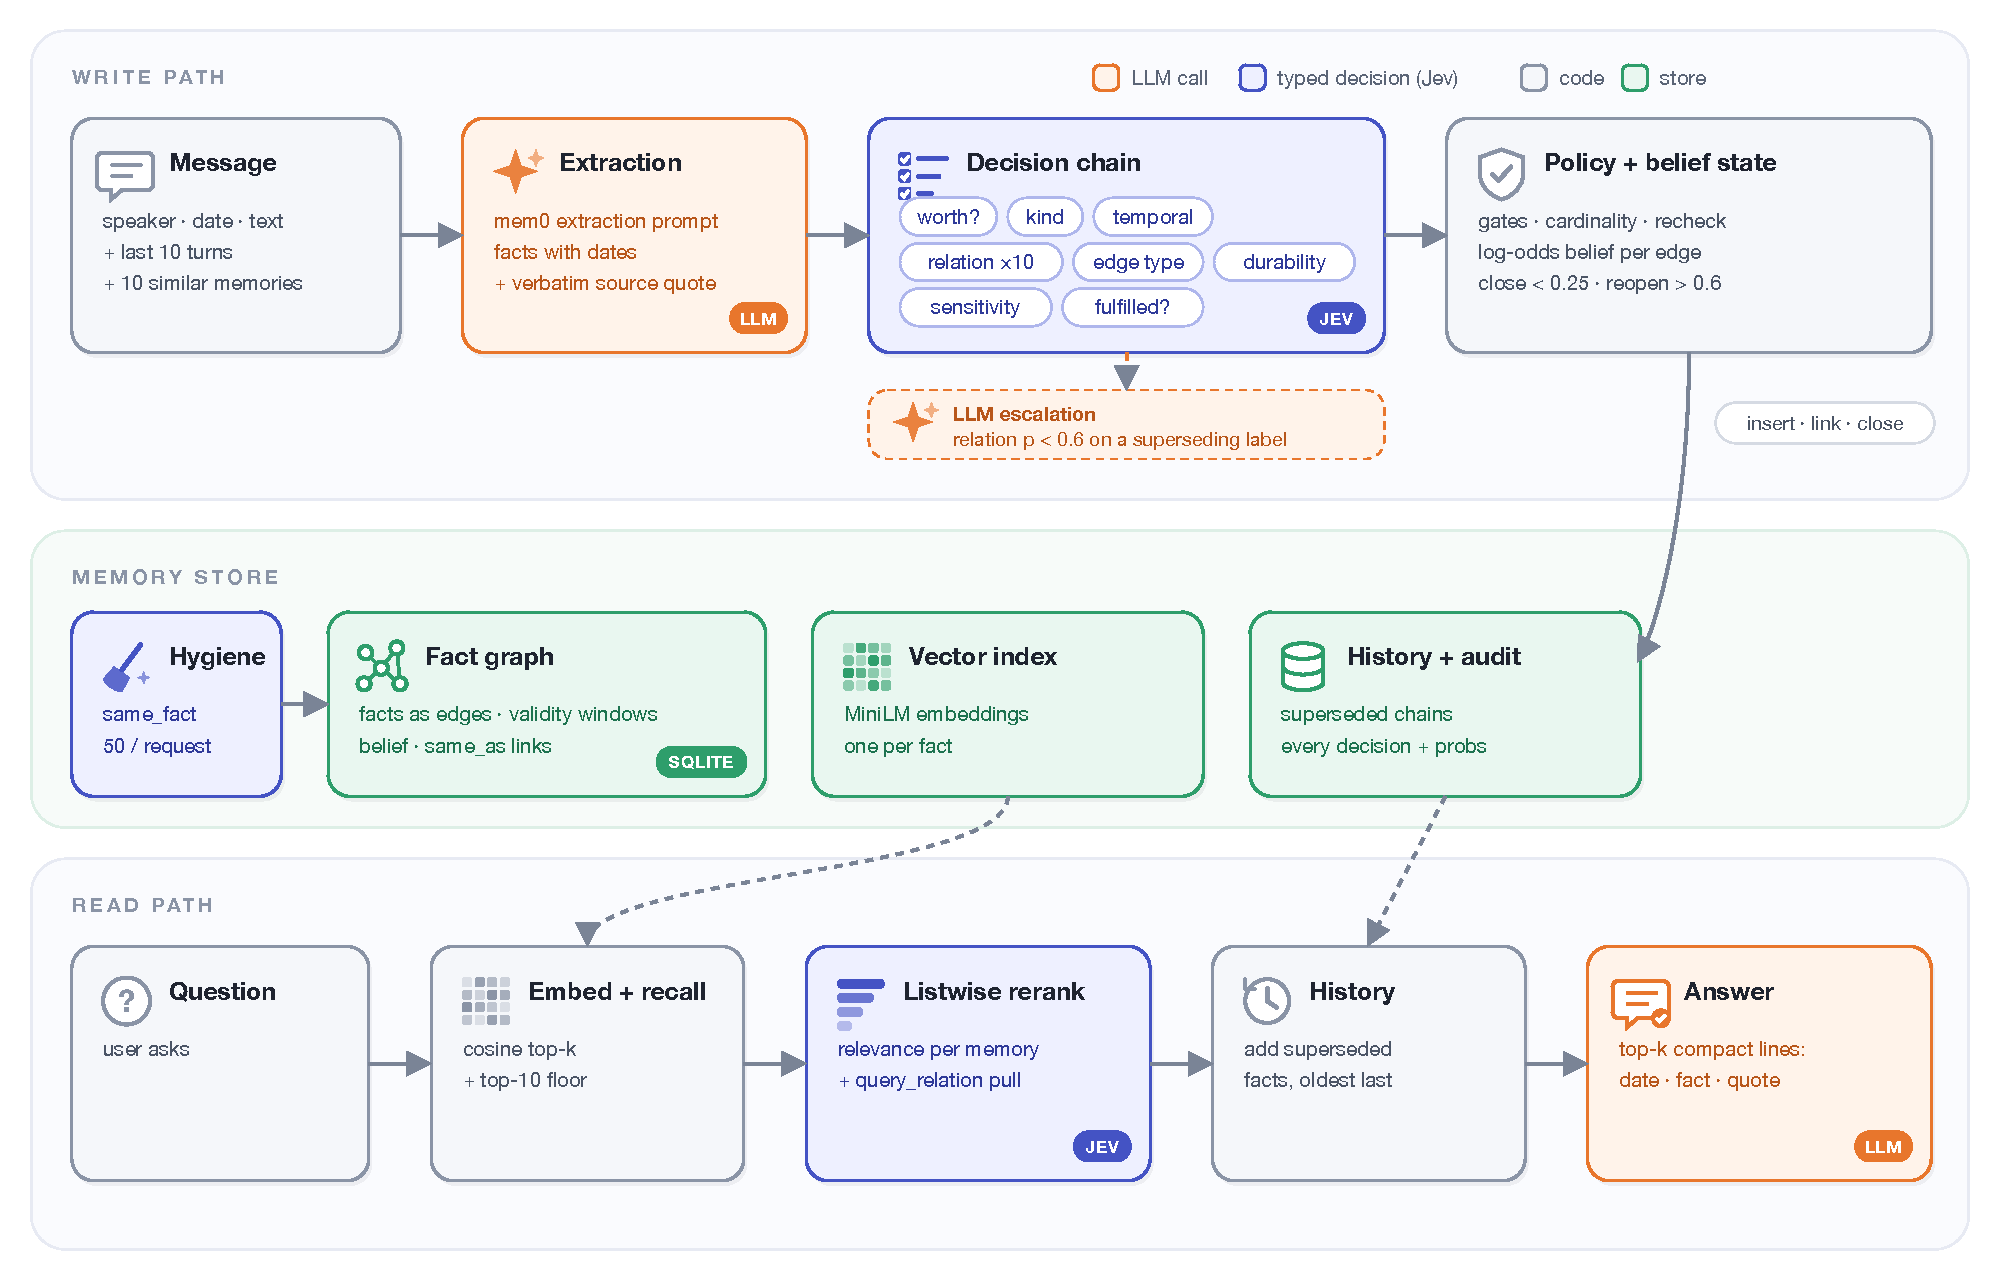
\includegraphics[width=\textwidth]{figures/pipeline.pdf}
\caption{engram's write and read paths. Only extraction, the answer and the escalation of unsure superseding relations are LLM calls (orange); every other decision is a typed Jev question (blue).}\label{fig:1}
\end{figure*}
\textbf{Concurrent work.} The architectural idea of routing memory decisions to a typed decision model was reached independently by Jev-Mem \citep{jiang2026jevmem}, which uses Jev for typing, relation construction, query routing, budget allocation, traversal, candidate scoring and stopping. It reports a LoCoMo judge score of 0.777\src{jiang2026jevmem (reported LoCoMo judge score)} with a 158\src{jiang2026jevmem (reported build time, s)} s build and 0.93\src{jiang2026jevmem (reported query time, s)} s query against A-MEM \citep{xu2025amem}, MAGMA \citep{jiang2026magma} and two further systems reported in that paper. It does not isolate the decision layer, evaluate updates or closes, measure calibration, or use a held-out split or confidence intervals. Separately, a community article reranked AtMem's top-10 with Jev on 1,986\src{taghia2026atmem (LoCoMo questions)} LoCoMo questions and measured the effect at the ranking level: MRR@5 rose from 0.4259\src{taghia2026atmem (MRR@5, AtMem)} to 0.5868\src{taghia2026atmem (MRR@5, AtMem + Jev)} and Recall@1 from 0.3399\src{taghia2026atmem (Recall@1, AtMem)} to 0.5423\src{taghia2026atmem (Recall@1, AtMem + Jev)} \citep{taghia2026atmem}. This paper's contribution is the controlled measurement: an ablation of the decision layer using the same extraction model, prompt construction and implementation, its calibration, the behaviour of the store it drives, the retrieval effect on answers with a matched-context control and a held-out no-rerank arm, and a negative result.

\textbf{Contributions.} The paper makes three. First, typed decisions make re-examining the store affordable: engram writes at about add-only mem0's cost (\$9.90\src{bench/results/e2\_jev\_\_dev.json} against \$9.80\src{bench/results/mem0\_\_dev.json} per 1,000 messages on the dev slice, \$10.22\src{bench/results/heldout\_report.json} to \$10.55\src{bench/results/heldout\_report.json} against \$9.92\src{bench/results/heldout\_report.json} to \$10.16\src{bench/results/heldout\_report.json} held out). Against an LLM decider using the same extraction model, prompt construction and implementation, our claude-sonnet-4-6 implementation of mem0's update prompt with one call per extracted fact, typed decisions had 70.0$\times$\src{bench/results/e2\_llm\_\_dev.json ÷ bench/results/e2\_jev\_\_dev.json} lower decision cost and 27.6$\times$\src{bench/results/e2\_llm\_\_dev.json ÷ bench/results/e2\_jev\_\_dev.json} lower median decision latency, with equal accuracy on a 35\src{bench/results/e2\_jev\_\_dev.json}-question dev slice (\cref{sec:5.1}). The latency ratio excludes escalations: the Jev arm it measures made 0\src{bench/results/e2\_jev\_\_dev.json}. The frozen system escalates; on the held-out conversations its median decision latency was 868 ms\src{bench/results/heldout\_report.json} to 1,982 ms\src{bench/results/heldout\_report.json}, and its median end-to-end write was slower than mem0's on 3\src{bench/results/heldout\_report.json: conversations where engram's write p50 exceeds mem0's} of 4\src{bench/results/heldout\_report.json}. Second, a belief-state store policy with reversible, gated closes closed 0/8\src{bench/results/e4\_belief\_v2\_\_dev\_updates\_\_k3.json} no-close trap items, with 1\src{bench/results/e4\_belief\_v2\_\_dev\_updates\_\_k3.json} wrong plan\_fulfilled close and 1\src{bench/results/e4\_belief\_v2\_\_dev\_updates\_\_k3.json} close matching no labeled pair, and its v3 rule removes a weak-evidence failure that closes true facts (\cref{sec:3.2}, \cref{sec:5.3}). Third, on 610\src{bench/results/heldout\_report.json} held-out questions at a matched mean retrieved-context budget, engram was +8.7\src{bench/results/mem0\_token\_matched\_\_heldout\_pooled\_\_k6.json} points above mem0; turning Jev's reranking off costs 13.4\src{bench/results/heldout\_extra.json} points on the same questions and leaves engram at -4.8\src{bench/results/heldout\_extra.json} points against token-matched mem0, so on held-out data the reranker accounts for the whole difference (\cref{sec:5.2}). A negative result frames all three: closing stale facts did not change answers (\cref{sec:5.4}). Figure~\ref{fig:2} plots the third result against the context each system shows the answer model.

\begin{figure}[tbp]
\centering
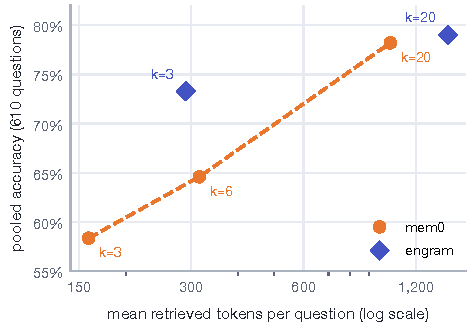
\includegraphics[width=\columnwidth]{figures/acc_vs_tokens.pdf}
\caption{Pooled held-out accuracy (610\src{bench/results/heldout\_report.json} questions) against $T(k)$, with per-question 95\% intervals; models as in Table~\ref{tab:2}. No line joins the points: mem0's accuracy was measured at $k{=}$3\src{bench/results/heldout\_report.json (k=3 run)}, 6\src{bench/results/mem0\_token\_matched\_\_heldout\_pooled\_\_k6.json} and 20\src{bench/results/heldout\_report.json (20 run)} only, and the token-matching sweep counted tokens at the other k without answering. engram at $k{=}$3\src{bench/results/heldout\_report.json (k=3 run)} sits above mem0 at $k{=}$6\src{bench/results/mem0\_token\_matched\_\_heldout\_pooled\_\_k6.json}, which shows the answer model slightly more tokens; with reranking off, engram falls below mem0 at the same budget; at $k{=}$20\src{bench/results/heldout\_report.json (k=20 run)} the two systems are indistinguishable.}\label{fig:2}
\end{figure}
\textbf{Scope.} We compare against one baseline (mem0 OSS 2.1.0) on one benchmark (LoCoMo: one development conversation and four held-out conversations, scoring four of its five question categories; adversarial is excluded from the primary comparison, following mem0's evaluation protocol, and reported separately in Table~\ref{tab:3}). We use update sets drafted and labeled with an AI assistant at the author's direction (\cref{sec:4.3}), and one hosted decision model (Jev, \texttt{jev-1.13.0}). We did not test Zep/Graphiti or Letta, LongMemEval, other extraction, answer or judge models, multi-user stores, or non-English text. Every finding, the negative result in particular, is about these LoCoMo-derived evaluations with this extraction, rendering and answer setup.

\section{Background and Related Work}\label{sec:2}
\subsection{Write decisions in existing systems}\label{sec:2.1}
mem0 \citep{chhikara2025mem0} extracts and consolidates facts with LLM calls. Version 2.1.0 extracts with one LLM call per message; the prompt receives the new message, the last 10\src{src/engram/flags.py (extract\_last\_k, as mem0 2.1.0)} messages and the 10\src{src/engram/config.py} most similar existing memories, and emits only additions. Its older update step, which asked an LLM to label each new fact as ADD, UPDATE, DELETE or NONE against existing memories, is still shipped as \texttt{DEFAULT\_\allowbreak{}UPDATE\_\allowbreak{}MEMORY\_\allowbreak{}PROMPT}. We use it as the LLM decision layer in \cref{sec:5.1}.

Other systems also decide with an LLM. Zep's Graphiti builds a temporal knowledge graph and resolves entities and invalidates edges with LLM calls \citep{rasmussen2025zep}. MemGPT, now Letta, manages memory tiers through LLM function calls \citep{packer2023memgpt}. A-MEM links notes with LLM-written attributes \citep{xu2025amem}, and MAGMA organizes memory as multiple graphs \citep{jiang2026magma}. ByteRover curates a hierarchical context with an LLM; its retrieval is a five-tier progressive strategy that answers most queries in under 100\src{nguyen2026byterover (sub-100 ms tier resolution)} ms without LLM calls and escalates to agentic reasoning only for novel questions \citep{nguyen2026byterover}.

\subsection{Typed decision models}\label{sec:2.2}
A typed decision model takes a shared \emph{state} (JSON) and a set of questions, and returns a probability distribution for each question. A question is a choice among named options, each with a rubric; a yes/no (``noul'') question; or a score.

\textbf{Jev.} We use Jev through TypeSafe's API: model \texttt{jev-1.13.0}, priced at 0.042\src{src/engram/config.py (USD per million input tokens)} USD per million input tokens as billed to our account (\texttt{src/\allowbreak{}engram/\allowbreak{}config.py}); the public documentation does not list a price. Its documentation gives a limit of 255\src{typesafe2026jev (max options per Choice)} options per choice question \citep{typesafe2026jev}. Its latency varies modestly with request size (\cref{sec:5.5}).

An open-weights model with the same request format, Laya, was tested zero-shot as an exploratory alternative; it is reported in \hyperref[app:D]{Appendix~D}.

\subsection{LoCoMo and its limits}\label{sec:2.3}
LoCoMo \citep{maharana2024locomo} contains long multi-session conversations with questions in five categories, of which we score four (adversarial is excluded from the primary comparison, following mem0's evaluation protocol; \cref{sec:4.1}). LongMemEval \citep{wu2025longmemeval} also evaluates long-term conversational memory; we used only LoCoMo.

\textbf{It barely tests updates.} In the first 215\src{bench/results/e2\_jev\_\_stress.json} messages of conv-26, an LLM labeler (claude-sonnet-4-6, prompt in \texttt{bench/\allowbreak{}stale.py}) found 2\src{bench/results/e0\_baseline\_\_stress.json} claims that a later message makes no longer true (\texttt{bench/\allowbreak{}slices/\allowbreak{}conv26\_\allowbreak{}superseded.json}).

\textbf{Public scores are not comparable.} Published LoCoMo scores for the same systems differ between the systems' own reports and third-party reports \citep{mem0blog2026benchmarks,byteroverblog2026benchmark}. We do not quote those numbers. All comparisons here run both systems under one protocol.

\subsection{Closest work and adjacent ideas}\label{sec:2.4}
\textbf{Jev-Mem and AtMem.} Jev-Mem \citep{jiang2026jevmem} is the closest design: Jev controls typing, relation construction, query routing, budget allocation, traversal, candidate scoring and stopping. The two designs differ in the store and in retrieval. Jev-Mem runs with admission filtering off and preserves every observation, so its store is never updated or closed; engram's store is governed by a close/belief policy with reversible closes and merges (\cref{sec:3.2}). Jev-Mem routes queries across multiple views; engram uses a single listwise rerank over cosine candidates plus a query-relation pull (\cref{sec:3.3}). The AtMem--Jev article \citep{taghia2026atmem} measured the rerank at the ranking level (Recall@10 unchanged; median batch latency 3.32\src{taghia2026atmem (median batch latency, s)} s) and reported no answer accuracy or intervals.

\textbf{Reranking and context.} Long contexts are used poorly by language models \citep{liu2024lost}, and LLMs rerank candidates well \citep{sun2023rankgpt}; spending compute on selecting context rather than adding more of it follows from both, and our rerank result is an instance.

\textbf{Routers.} Routers send queries to cheaper models \citep{ong2025routellm,chen2024frugalgpt}, and small classifiers act as guardrails \citep{inan2023llamaguard}. The escalation rule \cref{eq:zones} is a router of that kind.

\textbf{Calibration.} Temperature scaling \citep{guo2017calibration} and conformal prediction \citep{angelopoulos2021conformal} give principled thresholds for acting on a model's probability. The belief update \cref{eq:belief} uses probabilities as likelihoods, so it depends on calibration, which \cref{sec:5.3} measures.

\section{engram}\label{sec:3}
\subsection{Setup and notation}\label{sec:3.1}
A conversation is a sequence of messages $m_1, m_2, \ldots$, and $\operatorname{date}(m_t)$ is the time message $m_t$ was said. After message $t$ the store is $M_t = (F_t, V_t, I_t)$. $F_t$ is the set of facts, $V_t$ the entity nodes, and $I_t$ a vector index over fact texts. A fact $u \in F_t$ is an edge from its subject $\operatorname{subj}(u) \in V_t$ to an object node, labelled with a relation $\operatorname{rel}(u)$, and carries its text, the verbatim source quote, $\operatorname{date}$ of its message, a validity window whose end $\operatorname{valid\_until}(u)$ is empty while the fact holds, and a belief $b_u \in [b_{\min}, b_{\max}]$ that it is currently true, with $b_{\min}$ = 0.02\src{src/engram/config.py} and $b_{\max}$ = 0.98\src{src/engram/config.py}. $\operatorname{ent}(u)$ is the set of named entities in its text, and $\operatorname{card}(\rho) \in \{\text{one}, \text{many}\}$ says whether relation type $\rho$ is single- or multi-valued. $s_{\cos}(x, y)$ is the cosine similarity of their MiniLM embeddings in $I_t$, and $\operatorname{Top}_n s_{\cos}(x, \cdot)$ is the list of the $n$ facts most similar to $x$, most similar first.

A decision backend $D \in \{\text{Jev}, \text{LLM}\}$ answers typed questions. A typed question $Q$ has an option set $O_Q$; given state $s$, $P_D(o \mid s, Q)$ is the probability $D$ gives option $o \in O_Q$. Its decision is the argmax option and its confidence $\pi$ the largest probability. $X$ is the extraction call (an LLM with mem0's prompt) and $L$ an LLM call (escalation or answer). Five thresholds act on these probabilities, all read from \texttt{src/\allowbreak{}engram/\allowbreak{}config.py} and checked against this paper by \texttt{tests/\allowbreak{}test\_\allowbreak{}paper\_\allowbreak{}thresholds.py}: a decision acts at $\theta_{\text{act}}$ = 0.85\src{src/engram/config.py}, a superseding relation below $\theta_{\text{esc}}$ = 0.60\src{src/engram/config.py} is escalated, a retrieved fact is relevant above $\theta_{\text{rel}}$ = 0.5\src{src/engram/config.py}, and belief closes an edge below $\theta_{\text{close}}$ = 0.25\src{src/engram/config.py} and reopens it above $\theta_{\text{open}}$ = 0.60\src{src/engram/config.py}. $\tau_Q$ is a per-question temperature, which rescales probabilities as $P^{1/\tau_Q}$ renormalised; it is fitted to measure calibration (\cref{sec:5.3}) and is not applied on the write path.

On the read path, $q$ is a question, $k$ the retrieval budget (the answer model sees $k$ memory lines), and $T(k)$ the mean number of retrieved-context tokens per question at budget $k$. Two systems answer the same questions, so every comparison is paired: for question $i$, $d_i = \text{engram}_i - \text{mem0}_i$ with each term 1 if the judge marks the answer correct and 0 otherwise.

\subsection{Write path: decision chain and policy layer}\label{sec:3.2}
Figure~\ref{fig:1} shows both paths, with the equations below marked on its boxes. For message $m_t$:

\begin{align}
& F^{\text{new}}_t = X\bigl(m_t,\ m_{t-10}, \ldots, m_{t-1}, \nonumber\\
& \qquad \operatorname{Top}_{10}\, s_{\cos}(m_t, \cdot)\bigr) \label{eq:extract}
\end{align}
Extraction sees the new message, the last ten messages and the ten most similar stored facts, as mem0 2.1.0's \texttt{add()} does, so both systems extract from the same kind of prompt.

\begin{align}
& C(f) = \operatorname{Top}_{10}\, s_{\cos}(f, \cdot) \nonumber\\
& \quad \cup \operatorname{Top}_{10}\bigl\{u : \operatorname{subj}(u) = \operatorname{subj}(f) \nonumber\\
& \qquad\qquad \wedge \operatorname{rel}(u) = \operatorname{rel}(f) \nonumber\\
& \qquad\qquad \vee\ \operatorname{ent}(u) \cap \operatorname{ent}(f) \neq \emptyset\bigr\} \label{eq:cand}
\end{align}
The graph half finds stored facts about the same subject and relation, or sharing a rare named entity, that cosine similarity ranks too low; each half is capped at ten, closest first.

\begin{align}
& d_j(f) = \arg\max_{o \in O_j} P_D(o \mid f, Q_j), \nonumber\\
& \pi_j(f) = \max_{o \in O_j} P_D(o \mid f, Q_j) \label{eq:factq}
\end{align}
The fact questions (worth remembering, kind, temporal status, relation type, durability, sensitivity) go to $D$ in one request with the relation questions of the next equation, so a fact costs one call.

\begin{align}
& r(f,u) = \arg\max_{o \in R} P_D(o \mid f, u, Q_{\text{rel}}), \nonumber\\
& \pi(f,u) = \max_{o \in R} P_D(o \mid f, u, Q_{\text{rel}}), \nonumber\\
& u^{*} = \arg\max_{u \in C(f)}\, \max_{o \in R \setminus \{\text{new}\}} P_D(o \mid f, u, Q_{\text{rel}}) \label{eq:rel}
\end{align}
Here $R$ = \{new, duplicate, refinement, update, contradiction, negates\} and $S$ = \{update, contradiction, negates\} is the superseding subset; the write decision is about the candidate $u^{*}$ the new fact most likely relates to, with relation $r^{*} = r(f, u^{*})$ and confidence $\pi^{*}$ its largest non-new probability.

\begin{align}
& \text{act if } \pi^{*} \ge \theta_{\text{act}}; \nonumber\\
& r^{*} \leftarrow L(f, u^{*}) \text{ if } r^{*} \in S \wedge \pi^{*} < \theta_{\text{esc}}; \nonumber\\
& \text{tentative otherwise, or if } \pi_{\text{worth}}(f) < \theta_{\text{act}} \label{eq:zones}
\end{align}
Only the uncertain superseding decisions, the ones that could wrongly close a fact, pay for an LLM call.

\begin{align}
& g_T(f) = \mathbb{1}\bigl[P_D(\text{current} \mid f) \nonumber\\
& \qquad\qquad + P_D(\text{past} \mid f) \ge \theta_{\text{act}}\bigr] \label{eq:gtemp}
\end{align}
A planned or hypothetical statement never counts against a stored fact, and the gate sums current and past because Jev splits a completed change between them.

\begin{align}
& g_C(f,u) = \mathbb{1}[r = \text{negates}] \nonumber\\
& \ \vee \mathbb{1}\bigl[r = \text{update} \nonumber\\
& \qquad \wedge (\operatorname{card}(\operatorname{rel}(u)) = \text{one} \vee \operatorname{sib}(f,u))\bigr] \nonumber\\
& \ \vee \mathbb{1}\bigl[r = \text{contradiction} \wedge \operatorname{card}(\operatorname{rel}(u)) = \text{one} \nonumber\\
& \qquad\qquad \wedge \operatorname{sib}(f,u)\bigr] \label{eq:gcard}
\end{align}
With $r = r(f,u)$ and $\operatorname{sib}(f,u)$ meaning same subject and relation, a new value can replace an old one only where the relation holds one value at a time, so ``likes hiking'' does not close ``likes painting''.

\begin{align}
& g_A(f,u) = \mathbb{1}\bigl[r'(f,u) \in S \wedge \pi'(f,u) \ge \theta_{\text{act}}\bigr] \label{eq:gagree}
\end{align}
The first piece of evidence against a fact, and every update on a multi-valued relation, must be confirmed by a second phrasing of the relation question ($r'$, $\pi'$), so one misread answer cannot start a close.

\begin{align}
& e(f,u) = +\operatorname{logit} \pi(f,u) \nonumber\\
& \qquad\qquad \text{ if } r \in \{\text{duplicate}, \text{refinement}\}; \nonumber\\
& e(f,u) = -\operatorname{logit} \pi(f,u) - \operatorname{logit} \pi'(f,u) \nonumber\\
& \qquad\qquad \text{ if } r \in S \wedge g_T\, g_C\, g_A = 1; \nonumber\\
& e(f,u) = 0 \ \text{ otherwise} \label{eq:evid}
\end{align}
Answers become evidence in log-odds, and the recheck term appears only when the recheck was asked.

\begin{align}
& \operatorname{logit} b_u \leftarrow \operatorname{logit} b_u + e(f,u), \nonumber\\
& \operatorname{logit} b_f \leftarrow \operatorname{logit} b_f - \textstyle\sum_{u} \min\bigl(e(f,u), 0\bigr) \label{eq:belief}
\end{align}
Nothing irreversible happens on one answer: evidence accumulates on the stored fact, clipped to $[b_{\min}, b_{\max}]$, and the new fact, which starts at 0.5 if tentative and at $\pi^{*}$ otherwise, gains what the old one loses. In v2 (the held-out runs) every answer counts; v3 counts an answer only when $\pi(f,u) > 0.5$, so weak support cannot lower belief.

\begin{align}
& \operatorname{valid\_until}(u) \leftarrow \operatorname{date}(m_t) \text{ if } b_u < \theta_{\text{close}}, \nonumber\\
& \operatorname{valid\_until}(u) \leftarrow \varnothing \text{ if closed by belief} \nonumber\\
& \qquad\qquad \text{and } b_u > \theta_{\text{open}} \label{eq:hyst}
\end{align}
The gap between the two thresholds keeps a fact from flickering open and closed on alternating answers.

\begin{align}
& \operatorname{valid\_until}(u) \leftarrow \operatorname{date}(m_t) \text{ if} \nonumber\\
& \quad P_D(\text{yes} \mid f, u, Q_{\text{ful}}) \ge \theta_{\text{act}} \nonumber\\
& \quad \wedge \bigl(\operatorname{rel}(u) \in \{\text{plans}, \text{goal}\} \nonumber\\
& \qquad\quad \vee d_{\text{temporal}}(u) = \text{planned}\bigr) \label{eq:plan}
\end{align}
A plan ends when it happens, which the relation question does not ask, so a dedicated yes/no question decides it.

\begin{align}
& \operatorname{same\_as}(f, u^{*}) \text{ if } r^{*} = \text{duplicate} \nonumber\\
& \qquad \wedge \pi^{*} \ge \theta_{\text{act}} \wedge f \text{ not tentative}; \nonumber\\
& \text{hygiene: link } (u,v) \text{ if} \nonumber\\
& \qquad P_D(\text{duplicate} \mid u, v, Q_{\text{same}}) \ge \theta_{\text{act}}, \nonumber\\
& \qquad \text{unlink if } \le 1 - \theta_{\text{act}} \label{eq:links}
\end{align}
Duplicates are linked, never merged, so a wrong merge can be undone; after ingestion one hygiene pass re-asks every pair that shares subject and relation (the 30\src{src/engram/pipeline/hygiene.py (MAX\_GROUP)} most recent per group, 50\src{src/engram/pipeline/hygiene.py} pairs per request).

\begin{align}
& M_{t+1} = U\bigl(M_t,\ F^{\text{new}}_t,\ \{d_j(f), r(f,u)\}\bigr) \label{eq:write}
\end{align}
$U$ applies the equations above in order, plus two overrides decided by rule, not by $D$: an explicit request to remember sets $\pi_{\text{worth}} = 1$, and a credential is redacted before any decision or storage.

On the held-out conversations one hygiene pass made between 1,865\src{bench/results/e4\_belief\_v2\_\_heldout\_conv-30\_\_k3.json} and 5,446\src{bench/results/e4\_belief\_v2\_\_heldout\_conv-42\_\_k3.json} decisions, for between \$0.0112\src{bench/results/e4\_belief\_v2\_\_heldout\_conv-30\_\_k3.json} and \$0.0332\src{bench/results/e4\_belief\_v2\_\_heldout\_conv-42\_\_k3.json} (\cref{sec:5.3}). With LLM decisions, re-examining the store at that scale is what becomes unaffordable.

\begin{figure}[tbp]
\centering
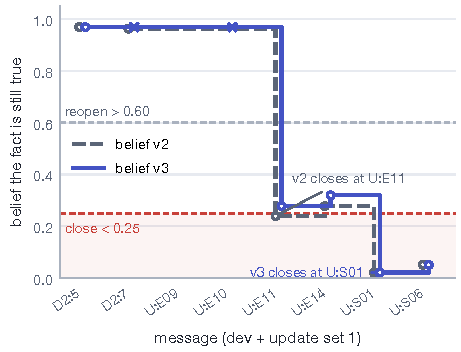
\includegraphics[width=\columnwidth]{figures/belief_trace.pdf}
\caption{Belief in the fact ``Melanie carves out daily me-time through running, reading, or playing violin'' (message D2:5), dev + update set 1, under v2 and v3. Source: the belief trace in \texttt{bench/\allowbreak{}results/\allowbreak{}e4\_\allowbreak{}belief\_\allowbreak{}v2\_\allowbreak{}\_\allowbreak{}dev\_\allowbreak{}updates\_\allowbreak{}\_\allowbreak{}k3\_\allowbreak{}\_\allowbreak{}noanswer.json} and its v3 counterpart. Under v2 the refinement answer at D2:7 ($\pi$ = 0.45\src{bench/results/e4\_belief\_v2\_\_dev\_updates\_\_k3\_\_noanswer.json (belief\_trace, D2:7)}) lowers belief slightly, so the update at U:E11 takes it below $\theta_{\text{close}}$; v3 ignores that answer ($\times$) and the fact closes one message later, at U:S01.}\label{fig:3}
\end{figure}
Figure~\ref{fig:3} traces one fact through \cref{eq:belief,eq:hyst} under both rules.

\subsection{Read path}\label{sec:3.3}
For question $q$ and budget $k$:

\begin{align}
& A(q) = \operatorname{Top}_{30}\, s_{\cos}(q, \cdot) \label{eq:short}
\end{align}
The shortlist includes closed facts, so a question about the past can reach them.

\begin{align}
& K(q) = \bigl[u \in A(q) : P_D(\text{yes} \mid u, q, Q_{\text{rlv}}) > \theta_{\text{rel}}\bigr] \nonumber\\
& \qquad \text{by } P_D(\text{yes} \mid u, q, Q_{\text{rlv}})\, b_u \text{ descending}, \nonumber\\
& \qquad \text{then the first ten of } A(q) \text{ not in } K(q) \label{eq:rerank}
\end{align}
One request scores every shortlisted fact, and the cosine floor keeps ten facts even when Jev judges few relevant.

\begin{align}
& g(q) = \arg\max_{g} P_D(g \mid q, Q_{\text{qr}}); \nonumber\\
& K(q) \leftarrow K(q) \cup \bigl\{u : \operatorname{rel}(u) = g(q)\bigr\} \nonumber\\
& \qquad \text{if } g(q) \neq \text{none} \wedge \max_{g} P_D(g \mid q, Q_{\text{qr}}) \ge \theta_{\text{act}} \label{eq:pull}
\end{align}
A question that names a relation (``where does she live?'') pulls in up to 10\src{src/engram/pipeline/retrieve.py (MAX\_RELATION\_PULL)} currently valid facts of that relation, which cosine similarity to the question may miss.

\begin{align}
& K^{+}(q) = K(q) \cup \textstyle\bigcup_{u \in K(q)} \operatorname{chain}(u) \cup N\bigl(K(q)\bigr) \label{eq:hist}
\end{align}
$\operatorname{chain}(u)$ is the facts $u$ superseded (linked through $\operatorname{valid\_until}$), so ``before Berlin'' finds Paris; $N$ adds up to 15\src{src/engram/pipeline/retrieve.py (MAX\_EXPANDED)} facts one hop from the kept facts' objects, skipping nodes with more than 25\src{src/engram/pipeline/retrieve.py (HUB\_DEGREE)} edges; a same\_as cluster is shown once.

\begin{align}
& a = L\bigl(q,\ \operatorname{render}(\text{first } k \text{ of } K^{+}(q))\bigr) \label{eq:answer}
\end{align}
Each line is the date the fact was said, the fact and its source quote, so the answer model can resolve recency itself. With reranking off, $K^{+}(q) = A(q)$ followed by its chains, so at $k$ = 3 the answer model sees the cosine top three.

\subsection{Cost model}\label{sec:3.4}
With a per-decision Jev cost $c_J$, an escalation cost $c_L$ and an escalation threshold $\theta$ on $\pi$:

\begin{align}
& C(\theta) = c_J + P(\pi < \theta)\, c_L \label{eq:cost}
\end{align}
Every decision pays for Jev, and only the escalated share pays for the LLM.

\begin{align}
& E(\theta) = P(\pi \ge \theta)\, \varepsilon_J(\theta) + P(\pi < \theta)\, \varepsilon_L \label{eq:error}
\end{align}
$\varepsilon_J(\theta)$ is Jev's error rate on the decisions it keeps and $\varepsilon_L$ the LLM's on the escalated ones, so raising $\theta$ trades cost for error only if $\varepsilon_L < \varepsilon_J$; \cref{sec:5.3} draws both curves.

\section{Experimental Setup}\label{sec:4}
\subsection{Models, data and protocol}\label{sec:4.1}
\textbf{Models.} Every arm uses the same models. \texttt{claude-haiku-4-5} extracts facts, for engram and for mem0 2.1.0 (which runs with telemetry off). \texttt{claude-sonnet-4-6} answers and judges, with mem0's LoCoMo evaluation prompts (\cref{sec:4.2}), and is also the LLM decision layer and the escalation model, with mem0's update prompt.

\textbf{Data.} The \emph{dev} slice is conv-26 sessions 1--4 (76\src{bench/results/e2\_jev\_\_dev.json} messages, 35\src{bench/results/e2\_jev\_\_dev.json} questions), and the \emph{stress} slice is conv-26 sessions 1--10 (215\src{bench/results/e2\_jev\_\_stress.json} messages, 80\src{bench/results/e2\_jev\_\_stress.json} questions). The \emph{held-out} slice is conv-30, conv-41, conv-42 and conv-43 whole (610\src{bench/results/heldout\_report.json} questions); none of it was used during development, and the system configuration was frozen (git tag \texttt{e4-frozen}) before any held-out run. LoCoMo's questions fall in five categories, of which we score four (adversarial is excluded from the primary comparison, following mem0's evaluation protocol). Each held-out conversation is ingested once per system, and $k{=}$3 and $k{=}$20 are answered from the same store.

\textbf{Caching and budget.} Every LLM and Jev call is cached by its full request, and budget guards stop any run past a spending limit. Phase 2 (all experiments reported here) spent \$101.79\src{bench/results/phase2\_spend.jsonl} over 84\src{bench/results/phase2\_spend.jsonl} ledgered runs. Jev accounts for \$1.51\src{bench/results/phase2\_spend.jsonl} of it (\texttt{bench/\allowbreak{}results/\allowbreak{}phase2\_\allowbreak{}spend.jsonl}; per-arm totals in \hyperref[app:E]{Appendix~E}). The build phase was not ledgered; roughly \$10 by the author's estimate.

\subsection{Shared extraction}\label{sec:4.2}
For each message, mem0 2.1.0's \texttt{add()} builds its extraction prompt from the new message (as \texttt{[date] speaker: text}), the last 10\src{src/engram/flags.py (extract\_last\_k, as mem0 2.1.0)} messages, the 10\src{src/engram/config.py} existing memories most similar to it, and a current date. It passes no observation date, so relative dates in historical conversations resolve against the current date. We report this as-is, and a patched variant in \cref{sec:6}.

engram's E-arms build the same prompt with the same function (\texttt{generate\_\allowbreak{}additive\_\allowbreak{}extraction\_\allowbreak{}prompt}), inputs and model (\texttt{bench/\allowbreak{}run.py}, \texttt{src/\allowbreak{}engram/\allowbreak{}flags.py}). The existing-memories input to extraction diverges once the two stores diverge, so extraction state is not identical across arms: replayed from the cache, the two E2 arms gave extraction different existing memories on 69\src{bench/results/e2\_extraction\_diff.json} of the 76\src{bench/results/e2\_extraction\_diff.json} dev messages (from message D1:8 on), and 26\src{bench/results/e2\_extraction\_diff.json} of the 76\src{bench/results/e2\_extraction\_diff.json} messages produced different extraction outputs between the Jev and LLM arms (\texttt{bench/\allowbreak{}e2\_\allowbreak{}extraction\_\allowbreak{}diff.py}). The E2 arms differ in what decides after extraction, and through it in the store that extraction reads.

\textbf{Prompts.} mem0's extraction and update prompts, and the functions that build their requests, are copied verbatim from the installed mem0 2.1.0 package (Apache License 2.0) into \texttt{src/\allowbreak{}engram/\allowbreak{}llm/\allowbreak{}prompts\_\allowbreak{}mem0.py}. \texttt{tests/\allowbreak{}test\_\allowbreak{}prompts\_\allowbreak{}mem0.py} checks that the copies are byte-identical to the installed package, so a changed prompt fails the test suite. The answer and judge prompts are mem0's LoCoMo evaluation prompts, adapted from two per-speaker memory lists to a single list (\texttt{bench/\allowbreak{}locomo\_\allowbreak{}subset.py}).

\subsection{Update sets}\label{sec:4.3}
LoCoMo has almost no updates (\cref{sec:2.3}). Two update sets, written in the speakers' voices, extend it. Both are appended to the dev slice and were frozen by SHA-256 before any run.

Set 1 (\texttt{bench/\allowbreak{}updates\_\allowbreak{}conv26.json}, SHA-256 prefix 2330876388f1\src{bench/updates\_conv26.json}) has 30\src{bench/updates\_conv26.json} items: 15\src{bench/updates\_conv26.json} easy closes, 10\src{bench/updates\_conv26.json} subtle items labeled \emph{no\_close} (past-tense mentions and unrealised plans that must not close anything), and 5\src{bench/updates\_conv26.json} fulfilled plans. Set 2 (\texttt{bench/\allowbreak{}updates2\_\allowbreak{}conv26.json}, prefix d4f3c8d2de61\src{bench/updates2\_conv26.json}) adds 28\src{bench/updates2\_conv26.json} messages and 20\src{bench/updates2\_conv26.json} questions. Of these, 5\src{bench/updates2\_conv26.json} ask about a past moment in set 1's items, 5\src{bench/updates2\_conv26.json} ask for the current value after a chain of 3--5 changes, 5\src{bench/updates2\_conv26.json} ask for a chain's value at a past moment, and 5\src{bench/updates2\_conv26.json} follow an update whose message has no temporal cue such as ``now'' or ``anymore''. \hyperref[app:B]{Appendix~B} shows one item of each kind; the full sets are in the two files. Update sets 1--2 were drafted and labeled with an AI assistant (Claude) at the author's direction; the author reviewed a subset. The 50 contradiction pairs were written and labeled by the author. This is a source of bias: the sets test failure modes the system's builders anticipated.

\subsection{Statistics}\label{sec:4.4}
Comparisons are paired over the same questions ($d_i$, \cref{sec:3.1}). We report an exact McNemar test on the discordant questions and a 95\% interval for the mean of $d_i$ from the per-question normal approximation. We also report a cluster bootstrap that resamples the four held-out conversations; with four clusters it is a robustness check, not a primary interval. Intervals are computed on the four scored categories, which stay the primary comparison.

\section{Results}\label{sec:5}
\subsection{Replacing the decision layer}\label{sec:5.1}
The three arms in Table~\ref{tab:1} share extraction. The two engram arms differ only in what decides after it: Jev's typed questions in E2 Jev, and \texttt{claude-sonnet-4-6} with mem0's update prompt, one call per extracted fact, in E2 LLM.

\begin{table*}[tbp]
\centering
\footnotesize\hyphenpenalty=10000\exhyphenpenalty=10000\setlength{\tabcolsep}{4.5pt}
\caption{Dev slice, conv-26 sessions 1--4, 76\src{bench/results/e2\_jev\_\_dev.json} messages, 35\src{bench/results/e2\_jev\_\_dev.json} questions, all retrieved memories (default k). Extraction claude-haiku-4-5 for all arms; answers and judge claude-sonnet-4-6; E2 LLM decides with claude-sonnet-4-6. Costs are per 1,000 messages written. Decision p50: median time after extraction, per message, over messages that produced at least one fact. Write p50: median end-to-end write time per message over all messages, including those that produced no facts. The two decision layers answer the same number of questions, while the Jev layer has 70.0$\times$\src{bench/results/e2\_llm\_\_dev.json ÷ bench/results/e2\_jev\_\_dev.json} lower decision cost and 27.6$\times$\src{bench/results/e2\_llm\_\_dev.json ÷ bench/results/e2\_jev\_\_dev.json} lower median decision latency than our claude-sonnet-4-6 implementation of mem0's update prompt, one call per extracted fact.}\label{tab:1}
\begin{tabular}{@{}>{\raggedright\arraybackslash}p{211.0pt}>{\raggedleft\arraybackslash}p{38.8pt}>{\raggedleft\arraybackslash}p{35.2pt}>{\raggedleft\arraybackslash}p{35.8pt}>{\raggedleft\arraybackslash}p{27.6pt}>{\raggedleft\arraybackslash}p{29.1pt}>{\raggedleft\arraybackslash}p{23.5pt}@{}}
\toprule
\textbf{system} & \textbf{accuracy} & \textbf{decision \$/1k} & \textbf{decision p50} & \textbf{total \$/1k} & \textbf{write p50} & \textbf{facts} \\
\midrule
mem0 2.1.0 (one LLM call per write) & 30/35\src{bench/results/mem0\_\_dev.json} & -- & -- & \$9.80\src{bench/results/mem0\_\_dev.json} & 879 ms\src{bench/results/mem0\_\_dev.json} & 46\src{bench/results/mem0\_\_dev.json} \\
engram E2, LLM decision layer (mem0 update prompt) & 31/35\src{bench/results/e2\_llm\_\_dev.json} & \$8.782\src{bench/results/e2\_llm\_\_dev.json} & 7,675 ms\src{bench/results/e2\_llm\_\_dev.json} & \$18.70\src{bench/results/e2\_llm\_\_dev.json} & 918 ms\src{bench/results/e2\_llm\_\_dev.json} & 18\src{bench/results/e2\_llm\_\_dev.json} \\
engram E2, Jev decision layer & 31/35\src{bench/results/e2\_jev\_\_dev.json} & \$0.125\src{bench/results/e2\_jev\_\_dev.json} & 278 ms\src{bench/results/e2\_jev\_\_dev.json} & \$9.90\src{bench/results/e2\_jev\_\_dev.json} & 895 ms\src{bench/results/e2\_jev\_\_dev.json} & 47\src{bench/results/e2\_jev\_\_dev.json} \\
\bottomrule
\end{tabular}
\end{table*}
On the 35\src{bench/results/e2\_jev\_\_dev.json}-question dev slice the two decision layers answer the same number of questions and mem0 one fewer, within noise. The Jev decision layer has 70.0$\times$\src{bench/results/e2\_llm\_\_dev.json ÷ bench/results/e2\_jev\_\_dev.json} lower decision cost and 27.6$\times$\src{bench/results/e2\_llm\_\_dev.json ÷ bench/results/e2\_jev\_\_dev.json} lower median decision latency than our claude-sonnet-4-6 implementation of mem0's update prompt, one call per extracted fact. The LLM decision layer stores fewer facts (18\src{bench/results/e2\_llm\_\_dev.json} against 47\src{bench/results/e2\_jev\_\_dev.json}) because mem0's UPDATE event rewrites an existing memory instead of adding one.

The two latency columns are medians over different messages. In the E2 LLM arm only 30\src{bench/results/e2\_latency.json} of 76\src{bench/results/e2\_latency.json} messages made an LLM decision call, so the write median falls on an extraction-only message (median extraction 869 ms\src{bench/results/e2\_latency.json}); on the messages with decisions, the logged median of the slowest decision call is 7,892 ms\src{bench/results/e2\_latency.json} (\texttt{bench/\allowbreak{}e2\_\allowbreak{}latency.py}).

In Table~\ref{tab:1} the decision layer is 1.3\%\src{bench/results/e2\_jev\_\_dev.json: decision $/1k ÷ total $/1k} of the Jev arm's end-to-end write cost and 47.0\%\src{bench/results/e2\_llm\_\_dev.json: decision $/1k ÷ total $/1k} of the LLM arm's; with typed decisions, extraction is almost the whole cost of a write, and engram writes at about add-only mem0's cost (\$9.90\src{bench/results/e2\_jev\_\_dev.json} against \$9.80\src{bench/results/mem0\_\_dev.json} per 1,000 messages) although mem0 never re-examines what it stored.

\textbf{Escalations and the frozen system.} Both ratios exclude escalations: the E2 Jev arm made 0\src{bench/results/e2\_jev\_\_dev.json} on the dev slice. The frozen system (\cref{sec:3.2}) escalates unsure superseding relations and asks more questions per fact; on the held-out conversations it escalated 31\src{bench/results/e4\_belief\_v2\_\_heldout\_conv-*\_\_k3.json} decisions, its median decision latency was 868 ms\src{bench/results/heldout\_report.json} to 1,982 ms\src{bench/results/heldout\_report.json} per conversation, and its median end-to-end write was slower than mem0's on 3\src{bench/results/heldout\_report.json: conversations where engram's write p50 exceeds mem0's} of 4\src{bench/results/heldout\_report.json} (Table~\ref{tab:12}, \hyperref[app:C]{Appendix~C}). Its write cost stayed close to mem0's (\$10.22\src{bench/results/heldout\_report.json} to \$10.55\src{bench/results/heldout\_report.json} against \$9.92\src{bench/results/heldout\_report.json} to \$10.16\src{bench/results/heldout\_report.json} per 1,000 messages).

The ratios are specific to that comparator: batching several facts per LLM call and a smaller LLM decider were not measured. On the stress slice the Jev arm scored 67/80\src{bench/results/e2\_jev\_\_stress.json} and mem0 64/80\src{bench/results/mem0\_\_stress.json}; the LLM arm was not run there.

\textbf{At $k{=}$20 the two systems are indistinguishable.} The held-out runs compare the frozen full system (E4 belief v2, \cref{sec:3.2}) with mem0, not the E2 arms. At $k{=}$20 engram answers 482/610\src{bench/results/heldout\_report.json} and mem0 477/610\src{bench/results/heldout\_report.json}. The difference is +0.8\src{bench/results/heldout\_report.json} points (95\% CI -2.3\src{bench/results/heldout\_report.json} to +3.9\src{bench/results/heldout\_report.json}; conversation bootstrap -4.5\src{bench/results/heldout\_report.json} to +5.4\src{bench/results/heldout\_report.json}; McNemar $p$ = 0.679\src{bench/results/heldout\_report.json}), within noise.

\subsection{Retrieval under a small budget}\label{sec:5.2}
Our answer-level result is consistent with the ranking-level improvement AtMem measured when reranking with Jev \citep{taghia2026atmem}.

At $k{=}$3 engram shows the answer model $T(3)$ = 290\src{bench/results/heldout\_report.json} tokens per question and mem0 159\src{bench/results/heldout\_report.json}. Most of the difference is the source quote on each engram line. To separate context size from ranking, we answered the same 610\src{bench/results/heldout\_report.json} questions from mem0's existing held-out stores at every k from 3 to 8. The token-matched setting is the k whose mean retrieved tokens came closest to engram's 290\src{bench/results/mem0\_token\_matched\_\_heldout\_pooled\_\_k6.json}: $k{=}$6\src{bench/results/mem0\_token\_matched\_\_heldout\_pooled\_\_k6.json}, at 315\src{bench/results/mem0\_token\_matched\_\_heldout\_pooled\_\_k6.json} tokens. That gives mem0 slightly more context than engram. The run cost \$2.52\src{bench/results/mem0\_token\_matched\_\_heldout\_pooled\_\_k6.json}.

\begin{table*}[tbp]
\centering
\footnotesize\hyphenpenalty=10000\exhyphenpenalty=10000\setlength{\tabcolsep}{3.5pt}
\caption{Held-out LoCoMo accuracy, pooled over conv-30, 41, 42 and 43 (610\src{bench/results/heldout\_report.json} questions, adversarial category excluded). Each row after an engram row carries its paired difference against engram at the same budget (engram $k{=}$3 for the $k{=}$3, reranking-off and token-matched rows, engram $k{=}$20 for the $k{=}$20 row); $\Delta$ is engram minus the row. Extraction claude-haiku-4-5, answers and judge claude-sonnet-4-6; one ingestion per system per conversation. Tokens: $T(k)$. 95\% CI: per-question normal approximation; bootstrap: resampling the four conversations. Discordant: questions only the engram row / only this row answered correctly. engram leads token-matched mem0 at $k{=}$3, turning reranking off costs more than that lead, and at $k{=}$20 the two systems are indistinguishable.}\label{tab:2}
\begin{tabular}{@{}>{\raggedright\arraybackslash}p{91.1pt}>{\raggedright\arraybackslash}p{19.9pt}>{\raggedleft\arraybackslash}p{35.0pt}>{\raggedleft\arraybackslash}p{38.8pt}>{\raggedleft\arraybackslash}p{23.6pt}>{\raggedleft\arraybackslash}p{54.9pt}>{\raggedleft\arraybackslash}p{50.4pt}>{\raggedleft\arraybackslash}p{44.2pt}>{\raggedleft\arraybackslash}p{41.0pt}@{}}
\toprule
\textbf{system} & \textbf{k} & \textbf{tokens/q} & \textbf{accuracy} & \textbf{$\Delta$ (pts)} & \textbf{95\% CI} & \textbf{95\% CI, bootstrap} & \textbf{discordant} & \textbf{McNemar p} \\
\midrule
engram & 3 & 290\src{bench/results/heldout\_report.json} & 73.3\%\src{bench/results/heldout\_report.json} & -- & -- & -- & -- & -- \\
mem0 & 3 & 159\src{bench/results/heldout\_report.json} & 58.4\%\src{bench/results/heldout\_report.json} & +14.9\src{bench/results/heldout\_report.json} & [+11.2\src{bench/results/heldout\_report.json},~+18.7\src{bench/results/heldout\_report.json}] & [+8.2\src{bench/results/heldout\_report.json},~+19.8\src{bench/results/heldout\_report.json}] & 120\src{bench/results/heldout\_report.json} / 29\src{bench/results/heldout\_report.json} & 2.4e-14\src{bench/results/heldout\_report.json} \\
engram, reranking off & 3 & 282\src{bench/results/heldout\_extra.json} & 59.8\%\src{bench/results/heldout\_extra.json} & +13.4\src{bench/results/heldout\_extra.json} & [+10.1\src{bench/results/heldout\_extra.json},~+16.8\src{bench/results/heldout\_extra.json}] & [+8.7\src{bench/results/heldout\_extra.json},~+17.8\src{bench/results/heldout\_extra.json}] & 101\src{bench/results/heldout\_extra.json} / 19\src{bench/results/heldout\_extra.json} & 1.1e-14\src{bench/results/heldout\_extra.json} \\
mem0 (token-matched) & 6\src{bench/results/mem0\_token\_matched\_\_heldout\_pooled\_\_k6.json} & 315\src{bench/results/mem0\_token\_matched\_\_heldout\_pooled\_\_k6.json} & 64.6\%\src{bench/results/mem0\_token\_matched\_\_heldout\_pooled\_\_k6.json} & +8.7\src{bench/results/heldout\_extra.json} & [+5.2\src{bench/results/heldout\_extra.json},~+12.1\src{bench/results/heldout\_extra.json}] & [+2.4\src{bench/results/heldout\_extra.json},~+14.7\src{bench/results/heldout\_extra.json}] & 86\src{bench/results/heldout\_extra.json} / 33\src{bench/results/heldout\_extra.json} & 1.3e-06\src{bench/results/heldout\_extra.json} \\
engram & 20 & 1,461\src{bench/results/heldout\_report.json} & 79.0\%\src{bench/results/heldout\_report.json} & -- & -- & -- & -- & -- \\
mem0 & 20 & 1,024\src{bench/results/heldout\_report.json} & 78.2\%\src{bench/results/heldout\_report.json} & +0.8\src{bench/results/heldout\_report.json} & [-2.3\src{bench/results/heldout\_report.json},~+3.9\src{bench/results/heldout\_report.json}] & [-4.5\src{bench/results/heldout\_report.json},~+5.4\src{bench/results/heldout\_report.json}] & 49\src{bench/results/heldout\_report.json} / 44\src{bench/results/heldout\_report.json} & 0.679\src{bench/results/heldout\_report.json} \\
\bottomrule
\end{tabular}
\end{table*}
Table~\ref{tab:2} has the pooled results. At $k{=}$3 engram is ahead of mem0 by +14.9\src{bench/results/heldout\_report.json} points (95\% CI +11.2\src{bench/results/heldout\_report.json} to +18.7\src{bench/results/heldout\_report.json}). At a matched mean retrieved-context budget, engram was +8.7\src{bench/results/mem0\_token\_matched\_\_heldout\_pooled\_\_k6.json} points above mem0 (95\% CI +5.2\src{bench/results/mem0\_token\_matched\_\_heldout\_pooled\_\_k6.json} to +12.1\src{bench/results/mem0\_token\_matched\_\_heldout\_pooled\_\_k6.json}; conversation bootstrap +2.4\src{bench/results/heldout\_extra.json} to +14.7\src{bench/results/heldout\_extra.json}; McNemar p-value 1.3e-06\src{bench/results/mem0\_token\_matched\_\_heldout\_pooled\_\_k6.json}; 86\src{bench/results/mem0\_token\_matched\_\_heldout\_pooled\_\_k6.json} questions only engram answered against 33\src{bench/results/mem0\_token\_matched\_\_heldout\_pooled\_\_k6.json} only mem0 answered). Figure~\ref{fig:2} places every measured setting on one axis of $T(k)$.

engram's point estimate is ahead of token-matched mem0 in each of the four scored categories (Table~\ref{tab:3}) and in every conversation (\hyperref[app:C]{Appendix~C}). Per conversation, the matched-context interval excludes zero in 2\src{bench/results/perconv\_diffs.json: conversations whose matched-context interval excludes zero} of four conversations (conv-42 and conv-43); conv-30 and conv-41 are within noise on their own.

Table~\ref{tab:3} adds LoCoMo's adversarial category, 190\src{bench/results/heldout\_extra.json} questions about things the conversations never say, whose gold answer is to abstain. Our intervals are computed on the four scored categories, which stay the primary comparison. engram with reranking scores lowest on adversarial questions at both budgets (71.1\%\src{bench/results/heldout\_extra.json} at $k{=}$3, 67.9\%\src{bench/results/heldout\_extra.json} at $k{=}$20, against 75.8\%\src{bench/results/heldout\_extra.json} for token-matched mem0 and 76.3\%\src{bench/results/heldout\_extra.json} with reranking off); over all five categories engram $k{=}$3 scores 72.8\%\src{bench/results/heldout\_extra.json} and token-matched mem0 67.2\%\src{bench/results/heldout\_extra.json}. We did not test why; the answer prompt does not ask for abstention, and a context of relevant memories may invite an answer.

\begin{table*}[tbp]
\centering
\footnotesize\hyphenpenalty=10000\exhyphenpenalty=10000\setlength{\tabcolsep}{4.5pt}
\caption{LoCoMo, four held-out conversations, LLM-as-a-judge with mem0's judge prompt on claude-sonnet-4-6; extraction claude-haiku-4-5, answers claude-sonnet-4-6. Adversarial gold answers require abstention, which mem0's answer prompt does not instruct; both systems share that handicap. Scores are not comparable to leaderboards run on other model stacks. engram at $k{=}$3 is ahead of token-matched mem0 in all four scored categories and behind every mem0 setting on adversarial questions.}\label{tab:3}
\begin{tabular}{@{}>{\raggedright\arraybackslash}p{123.8pt}>{\raggedleft\arraybackslash}p{41.9pt}>{\raggedleft\arraybackslash}p{43.2pt}>{\raggedleft\arraybackslash}p{57.2pt}>{\raggedleft\arraybackslash}p{48.2pt}>{\raggedleft\arraybackslash}p{52.2pt}>{\raggedleft\arraybackslash}p{34.2pt}@{}}
\toprule
\textbf{method} & \textbf{Multi-Hop} & \textbf{Temporal} & \textbf{Open-Domain} & \textbf{Single-Hop} & \textbf{Adversarial} & \textbf{Overall} \\
\midrule
questions & 110\src{bench/results/heldout\_extra.json} & 119\src{bench/results/heldout\_extra.json} & 33\src{bench/results/heldout\_extra.json} & 348\src{bench/results/heldout\_extra.json} & 190\src{bench/results/heldout\_extra.json} & 800\src{bench/results/heldout\_extra.json} \\
engram $k{=}$3 & 49.1\%\src{bench/results/heldout\_extra.json} & 84.0\%\src{bench/results/heldout\_extra.json} & 51.5\%\src{bench/results/heldout\_extra.json} & 79.3\%\src{bench/results/heldout\_extra.json} & 71.1\%\src{bench/results/heldout\_extra.json} & 72.8\%\src{bench/results/heldout\_extra.json} \\
engram $k{=}$3, reranking off & 31.8\%\src{bench/results/heldout\_extra.json} & 75.6\%\src{bench/results/heldout\_extra.json} & 33.3\%\src{bench/results/heldout\_extra.json} & 65.8\%\src{bench/results/heldout\_extra.json} & 76.3\%\src{bench/results/heldout\_extra.json} & 63.7\%\src{bench/results/heldout\_extra.json} \\
mem0 $k{=}$3 & 31.8\%\src{bench/results/heldout\_extra.json} & 71.4\%\src{bench/results/heldout\_extra.json} & 30.3\%\src{bench/results/heldout\_extra.json} & 64.9\%\src{bench/results/heldout\_extra.json} & 75.3\%\src{bench/results/heldout\_extra.json} & 62.4\%\src{bench/results/heldout\_extra.json} \\
mem0 $k{=}$6 (token-matched) & 40.9\%\src{bench/results/heldout\_extra.json} & 73.9\%\src{bench/results/heldout\_extra.json} & 33.3\%\src{bench/results/heldout\_extra.json} & 71.8\%\src{bench/results/heldout\_extra.json} & 75.8\%\src{bench/results/heldout\_extra.json} & 67.2\%\src{bench/results/heldout\_extra.json} \\
engram $k{=}$20 & 67.3\%\src{bench/results/heldout\_extra.json} & 88.2\%\src{bench/results/heldout\_extra.json} & 51.5\%\src{bench/results/heldout\_extra.json} & 82.2\%\src{bench/results/heldout\_extra.json} & 67.9\%\src{bench/results/heldout\_extra.json} & 76.4\%\src{bench/results/heldout\_extra.json} \\
mem0 $k{=}$20 & 61.8\%\src{bench/results/heldout\_extra.json} & 84.0\%\src{bench/results/heldout\_extra.json} & 57.6\%\src{bench/results/heldout\_extra.json} & 83.3\%\src{bench/results/heldout\_extra.json} & 75.3\%\src{bench/results/heldout\_extra.json} & 77.5\%\src{bench/results/heldout\_extra.json} \\
\bottomrule
\end{tabular}
\end{table*}
\textbf{Attribution.} Matching context removes 41.8\%\src{bench/results/heldout\_report.json and bench/results/mem0\_token\_matched\_\_heldout\_pooled\_\_k6.json: (Δk3 − Δtoken-matched) / Δk3} of the $k{=}$3 difference. What remains is a question of which memories are shown, which a held-out arm with Jev's reranking off answers (Table~\ref{tab:2}). From the same frozen stores, with the same answer and judge models, reranking off shows the answer model $T(3)$ = 282\src{bench/results/heldout\_extra.json} tokens, close to the full pipeline's, and answers 365/610\src{bench/results/heldout\_extra.json} (59.8\%\src{bench/results/heldout\_extra.json}). The full pipeline answers 13.4\src{bench/results/heldout\_extra.json} points more (95\% CI +10.1\src{bench/results/heldout\_extra.json} to +16.8\src{bench/results/heldout\_extra.json}; conversation bootstrap +8.7\src{bench/results/heldout\_extra.json} to +17.8\src{bench/results/heldout\_extra.json}; McNemar p-value 1.1e-14\src{bench/results/heldout\_extra.json}), and reranking off is -4.8\src{bench/results/heldout\_extra.json} points against token-matched mem0 (95\% CI -8.4\src{bench/results/heldout\_extra.json} to -1.1\src{bench/results/heldout\_extra.json}; McNemar p-value 0.014\src{bench/results/heldout\_extra.json}). On held-out data the reranker therefore accounts for the whole matched-context lead; without it, the rest of the pipeline (floor, relation pull, history, rendering) is below mem0 at the same budget. With reranking off the answer model sees the cosine top three \cref{eq:answer}. The store copies reproduced the frozen run's $k{=}$3 context for all but 3\src{bench/results/heldout\_extra.json} of the 610\src{bench/results/heldout\_report.json} questions (\texttt{bench/\allowbreak{}heldout\_\allowbreak{}extra.py}).

\subsection{Store behaviour and calibration}\label{sec:5.3}
\begin{table*}[tbp]
\centering
\footnotesize\hyphenpenalty=10000\exhyphenpenalty=10000\setlength{\tabcolsep}{3.5pt}
\caption{Store outcomes and update-question accuracy on the dev slice with update sets 1 and 2 (extraction claude-haiku-4-5, decisions Jev jev-1.13.0, answers and judge claude-sonnet-4-6). Closes are on dev + set 1, split by whether (closed fact's message, closing message) is a labeled update or superseded pair. Over-closed: set-1 no\_close items whose fact was closed by their own update message, over those stored. Stale: close items whose old fact is still active, over close items stored. Every arm kept the one set-2 keep item. Accuracy is at default k (all retrieved memories) unless marked; ``--'': run without answering or not run. No arm closed a no-close trap item (0/8 for every engram arm, 0/7 for mem0), and closing stale facts lowers the stale counts without moving update-question accuracy at default k, which is at or near ceiling for every arm that answered.}\label{tab:4}
\begin{tabular}{@{}>{\raggedright\arraybackslash}p{105.2pt}>{\raggedleft\arraybackslash}p{26.8pt}>{\raggedleft\arraybackslash}p{29.5pt}>{\raggedleft\arraybackslash}p{38.5pt}>{\raggedleft\arraybackslash}p{47.8pt}>{\raggedleft\arraybackslash}p{22.1pt}>{\raggedleft\arraybackslash}p{26.4pt}>{\raggedleft\arraybackslash}p{22.1pt}>{\raggedleft\arraybackslash}p{22.1pt}>{\raggedleft\arraybackslash}p{22.3pt}>{\raggedleft\arraybackslash}p{22.1pt}@{}}
\toprule
\textbf{arm} & \textbf{closes} & \textbf{labeled} & \textbf{unlabeled} & \textbf{over-closed} & \textbf{set-1 stale} & \textbf{set-2 stale} & \textbf{set-1 acc.} & \textbf{set-1 acc. $k{=}$3} & \textbf{set-1 acc. no dates} & \textbf{set-2 acc.} \\
\midrule
mem0 (add-only) & 0\src{bench/results/mem0\_\_dev\_updates.json} & 0\src{bench/results/mem0\_\_dev\_updates.json} & 0\src{bench/results/mem0\_\_dev\_updates.json} & 0/7\src{bench/results/mem0\_\_dev\_updates.json} & 18/18\src{bench/results/mem0\_\_dev\_updates.json} & 16/16\src{bench/results/mem0\_\_dev\_updates2.json} & 29/30\src{bench/results/mem0\_\_dev\_updates.json} & 25/30\src{bench/results/mem0\_\_dev\_updates\_\_k3.json} & 29/30\src{bench/results/mem0\_\_dev\_updates\_\_nodates.json} & 20/20\src{bench/results/mem0\_\_dev\_updates2.json} \\
E2: Jev, replace-on-update & 11\src{bench/results/e2\_jev\_v2\_\_dev\_updates\_\_k3.json} & 3\src{bench/results/e2\_jev\_v2\_\_dev\_updates\_\_k3.json} & 8\src{bench/results/e2\_jev\_v2\_\_dev\_updates\_\_k3.json} & 0/8\src{bench/results/e2\_jev\_v2\_\_dev\_updates\_\_k3.json} & 10/18\src{bench/results/e2\_jev\_v2\_\_dev\_updates\_\_k3.json} & 15/16\src{bench/results/e2\_jev\_v2\_\_dev\_updates2.json} & 30/30\src{bench/results/e2\_jev\_v2\_\_dev\_updates.json} & 30/30\src{bench/results/e2\_jev\_v2\_\_dev\_updates\_\_k3.json} & 30/30\src{bench/results/e2\_jev\_v2\_\_dev\_updates\_\_nodates.json} & 19/20\src{bench/results/e2\_jev\_v2\_\_dev\_updates2.json} \\
E3: structural rules & 3\src{bench/results/e3\_structural\_v3\_\_dev\_updates.json} & 2\src{bench/results/e3\_structural\_v3\_\_dev\_updates.json} & 1\src{bench/results/e3\_structural\_v3\_\_dev\_updates.json} & 0/8\src{bench/results/e3\_structural\_v3\_\_dev\_updates.json} & 17/18\src{bench/results/e3\_structural\_v3\_\_dev\_updates.json} & not run & -- & -- & -- & -- \\
E4: belief v1 & 3\src{bench/results/e4\_belief\_\_dev\_updates.json} & 2\src{bench/results/e4\_belief\_\_dev\_updates.json} & 1\src{bench/results/e4\_belief\_\_dev\_updates.json} & 0/8\src{bench/results/e4\_belief\_\_dev\_updates.json} & 17/18\src{bench/results/e4\_belief\_\_dev\_updates.json} & 15/16\src{bench/results/e4\_belief\_\_dev\_updates2.json} & 30/30\src{bench/results/e4\_belief\_\_dev\_updates.json} & 30/30\src{bench/results/e4\_belief\_\_dev\_updates\_\_k3.json} & 29/30\src{bench/results/e4\_belief\_\_dev\_updates\_\_nodates.json} & 19/20\src{bench/results/e4\_belief\_\_dev\_updates2.json} \\
E4: belief v2 (frozen) & 4\src{bench/results/e4\_belief\_v2\_\_dev\_updates\_\_k3.json} & 3\src{bench/results/e4\_belief\_v2\_\_dev\_updates\_\_k3.json} & 1\src{bench/results/e4\_belief\_v2\_\_dev\_updates\_\_k3.json} & 0/8\src{bench/results/e4\_belief\_v2\_\_dev\_updates\_\_k3.json} & 14/18\src{bench/results/e4\_belief\_v2\_\_dev\_updates\_\_k3.json} & 10/16\src{bench/results/e4\_belief\_v2\_shadow\_\_dev\_updates2\_\_k3.json} & 30/30\src{bench/results/e4\_belief\_v2\_full\_\_dev\_updates.json} & 30/30\src{bench/results/e4\_belief\_v2\_\_dev\_updates\_\_k3.json} & -- & 20/20\src{bench/results/e4\_belief\_v2\_full\_\_dev\_updates2.json} \\
E4: belief v3 & 4\src{bench/results/e4\_belief\_v3\_\_dev\_updates\_\_k3\_\_noanswer.json} & 2\src{bench/results/e4\_belief\_v3\_\_dev\_updates\_\_k3\_\_noanswer.json} & 2\src{bench/results/e4\_belief\_v3\_\_dev\_updates\_\_k3\_\_noanswer.json} & 0/8\src{bench/results/e4\_belief\_v3\_\_dev\_updates\_\_k3\_\_noanswer.json} & 14/18\src{bench/results/e4\_belief\_v3\_\_dev\_updates\_\_k3\_\_noanswer.json} & 10/16\src{bench/results/e4\_belief\_v3\_\_dev\_updates2\_\_k3\_\_noanswer.json} & -- & -- & -- & -- \\
\bottomrule
\end{tabular}
\end{table*}
Table~\ref{tab:4} lists, for each arm, its closes, over-closes and stale items together with its accuracy on the update questions, and Figure~\ref{fig:4} plots the store outcomes.

\begin{figure}[tbp]
\centering
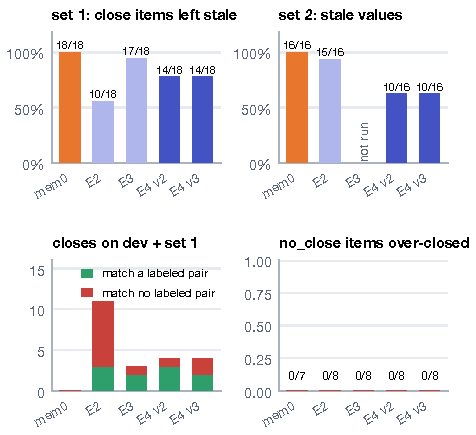
\includegraphics[width=\columnwidth]{figures/store_outcomes.pdf}
\caption{Store outcomes on the update sets: set-1 close items left stale, set-2 stale values, closes on dev + set 1 split by whether they match a labeled pair, and no\_close items over-closed. E3 was not run on set 2. The replace-on-update arm (E2) makes most of the closes that match no labeled pair; the belief arms close less and leave more set-1 items stale, and mem0 closes nothing.}\label{fig:4}
\end{figure}
\textbf{Trap items.} In the frozen arm 0/8\src{bench/results/e4\_belief\_v2\_\_dev\_updates\_\_k3.json} no-close trap items were closed, with 1\src{bench/results/e4\_belief\_v2\_\_dev\_updates\_\_k3.json} wrong plan\_fulfilled close and 1\src{bench/results/e4\_belief\_v2\_\_dev\_updates\_\_k3.json} close matching no labeled pair; no other arm closed a trap item either.

\textbf{Closes outside the labels.} These separate the policies. The first Jev arm (E2), which closed whenever a superseding label cleared 0.85\src{src/engram/config.py}, made 11\src{bench/results/e2\_jev\_v2\_\_dev\_updates\_\_k3.json} closes on dev + set 1, and 8\src{bench/results/e2\_jev\_v2\_\_dev\_updates\_\_k3.json} of them match no labeled pair. Belief v2 made 4\src{bench/results/e4\_belief\_v2\_\_dev\_updates\_\_k3.json}, of which 1\src{bench/results/e4\_belief\_v2\_\_dev\_updates\_\_k3.json} match no labeled pair. On set 2 the comparison is 10\src{bench/results/e2\_jev\_v2\_\_dev\_updates2.json} of 14\src{bench/results/e2\_jev\_v2\_\_dev\_updates2.json} against 1\src{bench/results/e4\_belief\_v2\_shadow\_\_dev\_updates2\_\_k3.json} of 10\src{bench/results/e4\_belief\_v2\_shadow\_\_dev\_updates2\_\_k3.json}.

\textbf{Stale items.} A stale item is a close item whose old fact is still active. Belief v2 left 14/18\src{bench/results/e4\_belief\_v2\_\_dev\_updates\_\_k3.json} of the set-1 close items stale, against 17/18\src{bench/results/e4\_belief\_\_dev\_updates.json} under belief v1 and 18/18\src{bench/results/mem0\_\_dev\_updates.json} for mem0, which never closes. On set 2 it left 10/16\src{bench/results/e4\_belief\_v2\_shadow\_\_dev\_updates2\_\_k3.json} stale, against 15/16\src{bench/results/e4\_belief\_\_dev\_updates2.json} and 16/16\src{bench/results/mem0\_\_dev\_updates2.json}.

\textbf{Fulfilled plans.} A relaxed heuristic closed a plan whenever a related past or current fact arrived. Across its two arms it fired 25\src{bench/results/e2\_jev\_v2\_\_dev\_updates.json + bench/results/e3\_structural\_v2\_\_dev\_updates.json (fulfills\_log) vs bench/updates\_conv26.json close\_fulfilled pairs} times. 1\src{bench/results/e2\_jev\_v2\_\_dev\_updates.json + bench/results/e3\_structural\_v2\_\_dev\_updates.json (fulfills\_log) vs bench/updates\_conv26.json close\_fulfilled pairs} firing matched a labeled (plan, fulfilment) pair, and 24\src{bench/results/e2\_jev\_v2\_\_dev\_updates.json + bench/results/e3\_structural\_v2\_\_dev\_updates.json (fulfills\_log) vs bench/updates\_conv26.json close\_fulfilled pairs} did not. The frozen arm uses the \texttt{plan\_\allowbreak{}fulfilled} question instead; it was asked 234\src{bench/results/e4\_belief\_v2\_\_dev\_updates\_\_k3.json} times on dev + set 1 and closed 2\src{bench/results/e4\_belief\_v2\_\_dev\_updates\_\_k3.json} plans correctly and 1\src{bench/results/e4\_belief\_v2\_\_dev\_updates\_\_k3.json} wrongly.

\textbf{Belief v3.} On the same data, v3 ignored 36\src{bench/results/e4\_belief\_v3\_\_dev\_updates\_\_k3\_\_noanswer.json} weak answers on dev + set 1 and 39\src{bench/results/e4\_belief\_v3\_\_dev\_updates2\_\_k3\_\_noanswer.json} with set 2 added. It closed the same four facts as v2 on dev + set 1. One of them, D2:5, crossed the close line at a different message (U:S01 rather than U:E11). Since that pair is not labeled, the audit scores v3 at 2\src{bench/results/e4\_belief\_v3\_\_dev\_updates\_\_k3\_\_noanswer.json} matching and 2\src{bench/results/e4\_belief\_v3\_\_dev\_updates\_\_k3\_\_noanswer.json} not matching, against v2's 3\src{bench/results/e4\_belief\_v2\_\_dev\_updates\_\_k3.json} and 1\src{bench/results/e4\_belief\_v2\_\_dev\_updates\_\_k3.json}. Stale and over-close counts are unchanged. v3 targets the weak-support failure that closed true facts under Laya (\hyperref[app:D]{Appendix~D}, exploratory).

\textbf{Hygiene.} One pass cost \$0.0015\src{bench/results/e4\_belief\_v2\_\_dev\_updates\_\_k3.json} on dev + set 1 (235\src{bench/results/e4\_belief\_v2\_\_dev\_updates\_\_k3.json} decisions). On the held-out conversations it cost \$0.0112\src{bench/results/e4\_belief\_v2\_\_heldout\_conv-30\_\_k3.json}, \$0.0254\src{bench/results/e4\_belief\_v2\_\_heldout\_conv-41\_\_k3.json}, \$0.0332\src{bench/results/e4\_belief\_v2\_\_heldout\_conv-42\_\_k3.json} and \$0.0323\src{bench/results/e4\_belief\_v2\_\_heldout\_conv-43\_\_k3.json}, making 9\src{bench/results/e4\_belief\_v2\_\_heldout\_conv-30\_\_k3.json}, 23\src{bench/results/e4\_belief\_v2\_\_heldout\_conv-41\_\_k3.json}, 32\src{bench/results/e4\_belief\_v2\_\_heldout\_conv-42\_\_k3.json} and 24\src{bench/results/e4\_belief\_v2\_\_heldout\_conv-43\_\_k3.json} links.

\textbf{Contradiction regression.} Table~\ref{tab:14} (\hyperref[app:D]{Appendix~D}) scores Jev on the regression set, next to Laya. The set has 50\src{bench/results/tradeoff.json} contradiction pairs, each an old fact, a new fact and a message, labeled with accepted relations and a temporal status (\texttt{bench/\allowbreak{}contradiction\_\allowbreak{}pairs.jsonl}). Under the current question versions, Jev's relation choice is in the accepted set for 90.0\%\src{bench/results/jev\_regression\_v2.json} of pairs (easy 100.0\%\src{bench/results/jev\_regression\_v2.json}, medium 93.3\%\src{bench/results/jev\_regression\_v2.json}, subtle 73.3\%\src{bench/results/jev\_regression\_v2.json}), and its temporal status is right for 94.0\%\src{bench/results/jev\_regression\_v2.json}. The write path's close rule is right for 76.0\%\src{bench/results/jev\_regression\_v2.json}, with 0\src{bench/results/jev\_regression\_v2.json} false closes. Jev's mean top probability is 0.88\src{bench/results/jev\_regression\_v2.json} when it is right and 0.81\src{bench/results/jev\_regression\_v2.json} when it is wrong.

\textbf{Calibration.} We measure calibration on two label sets: the 50\src{bench/results/tradeoff.json} gold pairs, and 29\src{bench/results/calibration.json} escalation labels, where Sonnet decided a relation Jev was unsure of. At these sizes expected calibration error (ECE) is exploratory, so Table~\ref{tab:5} also reports the Brier score and negative log-likelihood (NLL), both with bootstrap 95\% intervals. On the gold pairs Jev's relation NLL is 0.57\src{bench/results/calibration\_scores.json} (0.29\src{bench/results/calibration\_scores.json} to 0.89\src{bench/results/calibration\_scores.json}) and its relation ECE 0.14\src{bench/results/calibration.json} (fitted $\tau_Q$ = 1.48\src{bench/results/calibration.json}). On the escalation labels Jev's relation NLL is 3.18\src{bench/results/calibration\_scores.json} (0.38\src{bench/results/calibration\_scores.json} to 6.43\src{bench/results/calibration\_scores.json}): its mean confidence there is 0.92\src{bench/results/calibration.json}, so the relations it gets wrong it gets wrong with near-certain probability. Figure~\ref{fig:6} in \hyperref[app:C]{Appendix~C} has the reliability diagrams.

\begin{table*}[tbp]
\centering
\footnotesize\hyphenpenalty=10000\exhyphenpenalty=10000\setlength{\tabcolsep}{3.5pt}
\caption{Calibration of Jev (jev-1.13.0) on the escalation labels (dev + update sets, labels by claude-sonnet-4-6) and the gold contradiction pairs. ECE (exploratory at these n) uses 10 equal-width bins on the top choice; $\tau_Q$ is fitted by NLL per question and ``ECE at $\tau_Q$'' is out of sample (2-fold). Brier: sum over options of the squared error, averaged over items; NLL: $-\ln$ of the probability on the label; intervals: 10,000 bootstrap resamples of the items. Relation probabilities fold \texttt{negates} into \texttt{contradiction}, since the pairs predate \texttt{negates}. Laya's rows are in Table~\ref{tab:15} (\hyperref[app:D]{Appendix~D}). Jev's relation accuracy is about 80\% on both label sets; on the escalation labels its errors are confident, which raises its NLL.}\label{tab:5}
\begin{tabular}{@{}>{\raggedright\arraybackslash}p{40.5pt}>{\raggedright\arraybackslash}p{59.7pt}>{\raggedright\arraybackslash}p{36.5pt}>{\raggedleft\arraybackslash}p{10.9pt}>{\raggedleft\arraybackslash}p{25.1pt}>{\raggedleft\arraybackslash}p{22.6pt}>{\raggedleft\arraybackslash}p{21.3pt}>{\raggedleft\arraybackslash}p{23.5pt}>{\raggedleft\arraybackslash}p{21.3pt}>{\raggedleft\arraybackslash}p{61.8pt}>{\raggedleft\arraybackslash}p{61.8pt}@{}}
\toprule
\textbf{labels} & \textbf{question} & \textbf{backend} & \textbf{n} & \textbf{top-1 acc.} & \textbf{mean conf.} & \textbf{ECE} & \textbf{fitted $\tau$} & \textbf{ECE at $\tau$} & \textbf{Brier [95\% CI]} & \textbf{NLL [95\% CI]} \\
\midrule
escalation & relation & jev & 29\src{bench/results/calibration.json} & 79.3\%\src{bench/results/calibration.json} & 0.92\src{bench/results/calibration.json} & 0.15\src{bench/results/calibration.json} & 2.51\src{bench/results/calibration.json} & 0.10\src{bench/results/calibration.json} & 0.34\src{bench/results/calibration\_scores.json} [0.12\src{bench/results/calibration\_scores.json}, 0.61\src{bench/results/calibration\_scores.json}] & 3.18\src{bench/results/calibration\_scores.json} [0.38\src{bench/results/calibration\_scores.json}, 6.43\src{bench/results/calibration\_scores.json}] \\
gold pairs & relation & jev & 50\src{bench/results/calibration.json} & 82.0\%\src{bench/results/calibration.json} & 0.87\src{bench/results/calibration.json} & 0.14\src{bench/results/calibration.json} & 1.48\src{bench/results/calibration.json} & 0.14\src{bench/results/calibration.json} & 0.30\src{bench/results/calibration\_scores.json} [0.16\src{bench/results/calibration\_scores.json}, 0.46\src{bench/results/calibration\_scores.json}] & 0.57\src{bench/results/calibration\_scores.json} [0.29\src{bench/results/calibration\_scores.json}, 0.89\src{bench/results/calibration\_scores.json}] \\
gold pairs & temporal status & jev & 50\src{bench/results/calibration.json} & 94.0\%\src{bench/results/calibration.json} & 0.95\src{bench/results/calibration.json} & 0.04\src{bench/results/calibration.json} & 1.13\src{bench/results/calibration.json} & 0.04\src{bench/results/calibration.json} & 0.08\src{bench/results/calibration\_scores.json} [0.02\src{bench/results/calibration\_scores.json}, 0.17\src{bench/results/calibration\_scores.json}] & 0.14\src{bench/results/calibration\_scores.json} [0.04\src{bench/results/calibration\_scores.json}, 0.31\src{bench/results/calibration\_scores.json}] \\
\bottomrule
\end{tabular}
\end{table*}
\textbf{Cost/error tradeoff.} The 29\src{bench/results/calibration.json} escalation labels are too few for a curve, so Figure~\ref{fig:5} uses the 50\src{bench/results/tradeoff.json} gold pairs. The Jev cost $c_J$ = \$0.000016\src{bench/results/tradeoff.json} is the mean cost of one relation decision over 36,429\src{bench/results/tradeoff.json} held-out decisions, and the escalation cost $c_L$ = \$0.0073\src{bench/results/tradeoff.json} is the mean over 148\src{bench/results/tradeoff.json} logged escalations. No LLM run on the gold pairs is saved, so $\varepsilon_L$ is an assumption, plotted at 0 and 0.1. With Jev alone the error is 10.0\%\src{bench/results/tradeoff.json}. At $\theta$ = 0.85, 32.0\%\src{bench/results/tradeoff.json} of decisions escalate, the cost is \$0.002368\src{bench/results/tradeoff.json} per decision, and $E$ is 6.0\%\src{bench/results/tradeoff.json} ($\varepsilon_L$ = 0) or 9.2\%\src{bench/results/tradeoff.json} ($\varepsilon_L$ = 0.1). At the production threshold of 0.60\src{src/engram/config.py}, 8.0\%\src{bench/results/tradeoff.json} escalate and $E$ is 10.0\%\src{bench/results/tradeoff.json} or 10.8\%\src{bench/results/tradeoff.json}.

\begin{figure}[tbp]
\centering
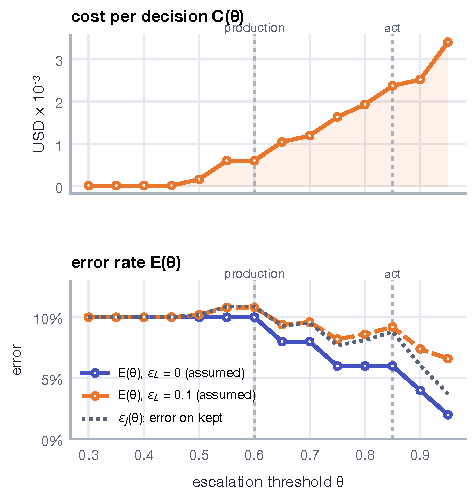
\includegraphics[width=\columnwidth]{figures/tradeoff.pdf}
\caption{$C(\theta)$ and $E(\theta)$ on the 50\src{bench/results/tradeoff.json} gold pairs. $\varepsilon_L$ is assumed, not measured; the 29\src{bench/results/calibration.json} escalation labels were too few for a curve. Error drops below Jev's own 10.0\%\src{bench/results/tradeoff.json} only where escalations make up almost all of the cost per decision, and how far it drops depends on an $\varepsilon_L$ we did not measure.}\label{fig:5}
\end{figure}
\subsection{Negative result: closes do not change answers}\label{sec:5.4}
\textbf{Closes do not change answers.} The accuracy columns of Table~\ref{tab:4} show it. mem0 never closes anything and leaves every set-1 close item stale (18/18\src{bench/results/mem0\_\_dev\_updates.json}), yet answers 29/30\src{bench/results/mem0\_\_dev\_updates.json} set-1 questions at default k. The arm that closes most aggressively leaves 10/18\src{bench/results/e2\_jev\_v2\_\_dev\_updates\_\_k3.json} stale and answers 30/30\src{bench/results/e2\_jev\_v2\_\_dev\_updates\_\_k3.json}.

The answer model resolves recency itself: extraction writes dates into the memory text, and the compact rendering adds the date each fact was said. Removing all dates, validity and source from the answer context (the no-dates column) still leaves every arm we ran that way at 29/30\src{bench/results/mem0\_\_dev\_updates\_\_nodates.json} or higher on set 1. Only the $k{=}$3 budget separates the systems (25/30\src{bench/results/mem0\_\_dev\_updates\_\_k3.json} for mem0, 30/30\src{bench/results/e2\_jev\_v2\_\_dev\_updates\_\_k3.json} for engram), which is a retrieval effect (\cref{sec:5.2}), not a close effect.

Set 2, which asks about chains of changes and past moments, is at its ceiling for every arm. Current LoCoMo-style questions do not reward a correct store.

\subsection{Systems notes}\label{sec:5.5}
\textbf{Jev latency varies modestly with request size below 50 questions; run-to-run variation is larger.} Across 9,446\src{bench/results/jev\_latency.json} live Jev requests from 25\src{bench/results/jev\_latency.json} runs, median latency is between 222 ms\src{bench/results/jev\_latency.json} and 269 ms\src{bench/results/jev\_latency.json} for requests of 1 to 50 questions, and 371 ms\src{bench/results/jev\_latency.json} for 51--80. A least-squares fit gives 380 ms\src{bench/results/jev\_latency.json} plus 7.19\src{bench/results/jev\_latency.json} ms per question (Figure~\ref{fig:7} and Table~\ref{tab:11}, \hyperref[app:C]{Appendix~C}). For requests of 16--20 questions, the per-run median was between 212 ms\src{bench/results/jev\_latency.json: per-run median, 16–20-question requests, runs with ≥30 such requests} and 267 ms\src{bench/results/jev\_latency.json: per-run median, 16–20-question requests, runs with ≥30 such requests} in 12\src{bench/results/jev\_latency.json: runs with ≥30 16–20-question requests, excluding conv-30 and conv-41} runs, and 793 ms\src{bench/results/jev\_latency.json: per-run median, 16–20-question requests} and 607 ms\src{bench/results/jev\_latency.json: per-run median, 16–20-question requests} in the two held-out runs made during one slower period.

\textbf{Extraction dominates write cost.} On the held-out set, engram's write cost is \$10.22\src{bench/results/heldout\_report.json} to \$10.55\src{bench/results/heldout\_report.json} per 1,000 messages and mem0's is \$9.92\src{bench/results/heldout\_report.json} to \$10.16\src{bench/results/heldout\_report.json}. The decision layer is 3.3\%\src{bench/results/heldout\_report.json: decision $/1k ÷ write $/1k} to 4.8\%\src{bench/results/heldout\_report.json: decision $/1k ÷ write $/1k} of engram's (Table~\ref{tab:12}, \hyperref[app:C]{Appendix~C}).

\textbf{Read path.} Per held-out question, engram's read path makes one Jev request, which scores every shortlisted fact and classifies the question's relation. It cost \$0.00039\src{bench/results/read\_path.json} per question on average, and its median latency per conversation was between 292 ms\src{bench/results/read\_path.json} and 2,531 ms\src{bench/results/read\_path.json}, following the run-to-run variation above (Table~\ref{tab:13}, \hyperref[app:C]{Appendix~C}). mem0's read path is a local embedding and vector search with no API call; its latency was not logged. engram's longer memory lines also make the answer call dearer: \$0.00245\src{bench/results/read\_path.json} per question against \$0.00229\src{bench/results/read\_path.json} for mem0 at $k{=}$3.

\section{Discussion}\label{sec:6}
\textbf{What the decision layer buys, and what it does not.} Typed decisions buy lower cost and latency (\cref{sec:5.1}), an audit trail in which every decision carries probabilities and a question version, store operations that are reversible and gated (\cref{sec:5.3}), and a price at which re-examining the store is routine (\cref{sec:3.2}). They do not buy accuracy at $k{=}$20, where the two systems are indistinguishable (\cref{sec:5.1}), or accuracy on these update questions, where every arm is near its ceiling (\cref{sec:5.4}).

\textbf{Benchmarks do not see storage correctness.} A question about a fact that changed is answerable from a store that kept both versions, as long as the memories carry dates. An evaluation that rewards a correct store would score answers against validity windows, use small retrieval budgets in which a stale fact displaces a current one, store memories without dates, and ask about long chains of changes. Update set 2 targets the last of these, and every arm is at its ceiling on it.

\textbf{The reranker, not the context size.} Under a three-memory budget engram leads token-matched mem0 by +8.7\src{bench/results/mem0\_token\_matched\_\_heldout\_pooled\_\_k6.json} points, and turning Jev's reranking off removes that lead and more (13.4\src{bench/results/heldout\_extra.json} points). The two systems are indistinguishable at $k{=}$20. On adversarial questions the reranked context scores lowest (Table~\ref{tab:3}); an answer prompt that asks for abstention was not tested.

\section{Conclusion}\label{sec:7}
Typed decisions let engram re-examine its store at about the write cost of add-only mem0. Against an LLM decider using the same extraction model, prompt construction and implementation, they had 70.0$\times$\src{bench/results/e2\_llm\_\_dev.json ÷ bench/results/e2\_jev\_\_dev.json} lower decision cost and 27.6$\times$\src{bench/results/e2\_llm\_\_dev.json ÷ bench/results/e2\_jev\_\_dev.json} lower median decision latency, with equal accuracy on a 35\src{bench/results/e2\_jev\_\_dev.json}-question dev slice. On 610\src{bench/results/heldout\_report.json} held-out questions, at a matched mean retrieved-context budget engram was +8.7\src{bench/results/mem0\_token\_matched\_\_heldout\_pooled\_\_k6.json} points above mem0; turning Jev's reranking off removed that lead and left engram at -4.8\src{bench/results/heldout\_extra.json} points against mem0, so the reranker accounts for it. At $k{=}$20 the two systems are indistinguishable. Closing stale facts, the part of the design aimed at correctness, did not change answers on our update sets: current LoCoMo-style questions do not reward a correct store.

\section*{Limitations}
We make no claim beyond these LoCoMo-derived evaluations with this extraction, rendering and answer setup. The comparison has one baseline, mem0 OSS 2.1.0, on one benchmark, four held-out LoCoMo conversations. Update sets 1--2 were drafted and labeled with an AI assistant (Claude) at the author's direction; the author reviewed a subset. The 50 contradiction pairs were written and labeled by the author.

\textbf{A closed, versioned API.} Every decision comes from Jev \texttt{jev-1.13.0}, served by TypeSafe's hosted API; its weights are not public. A later version may decide differently, and if this version is withdrawn our results can be replayed from the call cache but not recomputed. Jev is the only decision model evaluated as the deciding backend, and the open-weights Laya was tested only as a zero-shot base checkpoint (\hyperref[app:D]{Appendix~D}).

\textbf{The judge is the answer model.} claude-sonnet-4-6 both answers and judges, so the judge may favour answers written the way it would write them, and we did not measure its agreement with human labels.

Extraction shares model, prompt construction and implementation but not state: the stores it reads diverge (\cref{sec:4.2}), and no arm froze extraction outputs across decision layers. mem0's open-source path gives no observation date, so relative dates resolve against the run date; we use it as shipped, and a variant with the session date patched in scored 31/35\src{bench/results/mem0\_dated\_\_dev.json} on dev against 30/35\src{bench/results/mem0\_\_dev.json} unpatched, within noise. Adversarial questions require abstention, which mem0's answer prompt does not ask for (Table~\ref{tab:3}).

\section*{AI Assistance}
Code, experiment orchestration and paper drafting were carried out with Claude (Anthropic) via Claude Code under the author's direction; the author designed the study, made every methodological decision, and is responsible for all claims.

\bibliography{references}
\appendix
\onecolumn
\FloatBarrier
\section{Decision questions}\label{app:A}
Table~\ref{tab:6} lists the 12\src{src/engram/decide/questions.py (ALL\_QUESTIONS)} questions in the current chain with their types and options. \texttt{edge\_\allowbreak{}type} and \texttt{query\_\allowbreak{}relation} choose among 25\src{src/engram/decide/questions.py (EDGE\_TYPES)} relation types. The instructions and the rubric for every option of every version are in \texttt{src/\allowbreak{}engram/\allowbreak{}decide/\allowbreak{}questions.py}, and the reasons for each version change are in \texttt{docs/\allowbreak{}DECISIONS.md}.

\begingroup\scriptsize
\begin{longtable}{>{\raggedright\arraybackslash}p{0.256\linewidth}>{\raggedright\arraybackslash}p{0.141\linewidth}>{\raggedright\arraybackslash}p{0.513\linewidth}}
\caption{Jev questions in the current chain (\texttt{src/\allowbreak{}engram/\allowbreak{}decide/\allowbreak{}questions.py}).}\label{tab:6}\\
\toprule
\textbf{question} & \textbf{type} & \textbf{options} \\
\midrule
\endfirsthead
\toprule
\textbf{question} & \textbf{type} & \textbf{options} \\
\midrule
\endhead
\texttt{worth\_\allowbreak{}\allowbreak{}remembering} & noul v1 & yes / no \\
\texttt{fact\_\allowbreak{}\allowbreak{}kind} & choice v1 & \texttt{preference}, \texttt{bio}, \texttt{event}, \texttt{relationship}, \texttt{task}, \texttt{opinion} \\
\texttt{temporal\_\allowbreak{}\allowbreak{}status} & choice v2 & \texttt{current}, \texttt{planned}, \texttt{past}, \texttt{hypothetical} \\
\texttt{relation\_\allowbreak{}\allowbreak{}to\_\allowbreak{}\allowbreak{}candidate} & choice v2 & \texttt{new}, \texttt{duplicate}, \texttt{update}, \texttt{contradiction}, \texttt{refinement}, \texttt{negates} \\
\texttt{relation\_\allowbreak{}\allowbreak{}to\_\allowbreak{}\allowbreak{}candidate\_\allowbreak{}\allowbreak{}recheck} & choice v2 & \texttt{new}, \texttt{duplicate}, \texttt{update}, \texttt{contradiction}, \texttt{refinement}, \texttt{negates} \\
\texttt{edge\_\allowbreak{}\allowbreak{}type} & choice v1 & 25\src{src/engram/decide/questions.py} relation types \\
\texttt{durability} & choice v1 & \texttt{permanent}, \texttt{long\_\allowbreak{}\allowbreak{}term}, \texttt{short\_\allowbreak{}\allowbreak{}lived} \\
\texttt{sensitivity} & choice v1 & \texttt{none}, \texttt{health}, \texttt{financial}, \texttt{relationship}, \texttt{credentials} \\
\texttt{plan\_\allowbreak{}\allowbreak{}fulfilled} & noul v1 & yes / no \\
\texttt{relevant\_\allowbreak{}\allowbreak{}to\_\allowbreak{}\allowbreak{}query} & noul v1 & yes / no \\
\texttt{query\_\allowbreak{}\allowbreak{}relation} & choice v1 & 25\src{src/engram/decide/questions.py} relation types \\
\texttt{same\_\allowbreak{}\allowbreak{}fact} & noul v1 & yes / no \\
\bottomrule
\end{longtable}
\endgroup
\FloatBarrier
\section{Update sets}\label{app:B}
\begingroup\scriptsize
\begin{longtable}{>{\raggedright\arraybackslash}p{0.047\linewidth}>{\raggedright\arraybackslash}p{0.071\linewidth}>{\raggedright\arraybackslash}p{0.178\linewidth}>{\raggedright\arraybackslash}p{0.178\linewidth}>{\raggedright\arraybackslash}p{0.178\linewidth}>{\raggedright\arraybackslash}p{0.178\linewidth}}
\caption{One item of each kind from the two update sets (\texttt{bench/\allowbreak{}updates\_\allowbreak{}conv26.json}, \texttt{bench/\allowbreak{}updates2\_\allowbreak{}conv26.json}).}\label{tab:7}\\
\toprule
\textbf{id} & \textbf{kind} & \textbf{earlier fact or message} & \textbf{update message(s)} & \textbf{question} & \textbf{gold} \\
\midrule
\endfirsthead
\toprule
\textbf{id} & \textbf{kind} & \textbf{earlier fact or message} & \textbf{update message(s)} & \textbf{question} & \textbf{gold} \\
\midrule
\endhead
E01 & set 1, easy close & Melanie's main creative outlet is painting, which relaxes her after a long day. & I haven't painted in weeks, honestly. Pottery is my main creative outlet now - I go to the studio three evenings a week. & What is Melanie's main creative outlet now? & Pottery (she has stopped painting) \\
S01 & set 1, subtle (no\_\allowbreak{}close) & Melanie has been married to her husband for 5 years. & Our first apartment after the wedding was so tiny - we still laugh about it. & Is Melanie still married? & Yes, married for 5 years \\
F01 & set 1, fulfilled plan & Caroline plans to continue her education. & I did it - I enrolled in a psychology certificate program at the community college. Classes start next week! & Has Caroline enrolled in a program to continue her education? & Yes, a psychology certificate program at the community college \\
C01q1 & set 2, chain & I just moved into a studio apartment downtown. & Moved again! I'm in a two-bedroom in Oak Park now, so there's room for a foster kid. $\rightarrow$ We finally found a house - I live in Evanston now. & Where does Caroline live now? & A house in Evanston \\
N01 & set 2, no temporal cue & My favorite coffee spot is Blue Door Caf\'{e}. & My favorite coffee spot is Grind House. & What is Caroline's favorite coffee spot? & Grind House \\
\bottomrule
\end{longtable}
\endgroup
\FloatBarrier
\section{Per-conversation and systems tables}\label{app:C}
\begin{table}[!htbp]
\centering
\footnotesize\hyphenpenalty=10000\exhyphenpenalty=10000\setlength{\tabcolsep}{4.5pt}
\caption{Held-out accuracy per conversation, $k{=}$3. Q per row; models as in Table~\ref{tab:2}.}\label{tab:8}
\begin{tabular}{@{}>{\raggedright\arraybackslash}p{140.7pt}>{\raggedleft\arraybackslash}p{28.5pt}>{\raggedleft\arraybackslash}p{44.7pt}>{\raggedleft\arraybackslash}p{44.5pt}>{\raggedleft\arraybackslash}p{57.9pt}>{\raggedleft\arraybackslash}p{44.7pt}>{\raggedleft\arraybackslash}p{40.2pt}@{}}
\toprule
\textbf{conv.} & \textbf{Q} & \textbf{engram} & \textbf{mem0} & \textbf{$\Delta$ (questions)} & \textbf{engram tokens / q} & \textbf{mem0 tokens / q} \\
\midrule
conv-30 & 81\src{bench/results/heldout\_report.json} & 59/81\src{bench/results/heldout\_report.json} & 55/81\src{bench/results/heldout\_report.json} & 4\src{bench/results/heldout\_report.json} & 285\src{bench/results/heldout\_report.json} & 154\src{bench/results/heldout\_report.json} \\
conv-41 & 152\src{bench/results/heldout\_report.json} & 113/152\src{bench/results/heldout\_report.json} & 89/152\src{bench/results/heldout\_report.json} & 24\src{bench/results/heldout\_report.json} & 297\src{bench/results/heldout\_report.json} & 161\src{bench/results/heldout\_report.json} \\
conv-42 & 199\src{bench/results/heldout\_report.json} & 150/199\src{bench/results/heldout\_report.json} & 111/199\src{bench/results/heldout\_report.json} & 39\src{bench/results/heldout\_report.json} & 292\src{bench/results/heldout\_report.json} & 163\src{bench/results/heldout\_report.json} \\
conv-43 & 178\src{bench/results/heldout\_report.json} & 125/178\src{bench/results/heldout\_report.json} & 101/178\src{bench/results/heldout\_report.json} & 24\src{bench/results/heldout\_report.json} & 283\src{bench/results/heldout\_report.json} & 153\src{bench/results/heldout\_report.json} \\
\bottomrule
\end{tabular}
\end{table}
\begin{table}[!htbp]
\centering
\footnotesize\hyphenpenalty=10000\exhyphenpenalty=10000\setlength{\tabcolsep}{6.0pt}
\caption{Held-out accuracy per conversation, engram $k{=}$3 against token-matched mem0 ($k{=}$6). Q per row; models as in Table~\ref{tab:2}.}\label{tab:9}
\begin{tabular}{@{}>{\raggedright\arraybackslash}p{184.0pt}>{\raggedleft\arraybackslash}p{40.3pt}>{\raggedleft\arraybackslash}p{56.5pt}>{\raggedleft\arraybackslash}p{56.3pt}>{\raggedleft\arraybackslash}p{69.7pt}@{}}
\toprule
\textbf{conv.} & \textbf{Q} & \textbf{engram $k{=}$3} & \textbf{mem0 $k{=}$6} & \textbf{$\Delta$ (questions)} \\
\midrule
conv-30 & 81\src{bench/results/heldout\_report.json} & 59/81\src{bench/results/heldout\_report.json} & 54/81\src{bench/results/mem0\_token\_matched\_\_heldout\_pooled\_\_k6.json} & 5\src{bench/results/mem0\_token\_matched\_\_heldout\_pooled\_\_k6.json} \\
conv-41 & 152\src{bench/results/heldout\_report.json} & 113/152\src{bench/results/heldout\_report.json} & 109/152\src{bench/results/mem0\_token\_matched\_\_heldout\_pooled\_\_k6.json} & 4\src{bench/results/mem0\_token\_matched\_\_heldout\_pooled\_\_k6.json} \\
conv-42 & 199\src{bench/results/heldout\_report.json} & 150/199\src{bench/results/heldout\_report.json} & 119/199\src{bench/results/mem0\_token\_matched\_\_heldout\_pooled\_\_k6.json} & 31\src{bench/results/mem0\_token\_matched\_\_heldout\_pooled\_\_k6.json} \\
conv-43 & 178\src{bench/results/heldout\_report.json} & 125/178\src{bench/results/heldout\_report.json} & 112/178\src{bench/results/mem0\_token\_matched\_\_heldout\_pooled\_\_k6.json} & 13\src{bench/results/mem0\_token\_matched\_\_heldout\_pooled\_\_k6.json} \\
\bottomrule
\end{tabular}
\end{table}
\begin{table}[!htbp]
\centering
\footnotesize\hyphenpenalty=10000\exhyphenpenalty=10000\setlength{\tabcolsep}{4.5pt}
\caption{Held-out accuracy per conversation, $k{=}$20. Q per row; models as in Table~\ref{tab:2}.}\label{tab:10}
\begin{tabular}{@{}>{\raggedright\arraybackslash}p{140.7pt}>{\raggedleft\arraybackslash}p{28.5pt}>{\raggedleft\arraybackslash}p{44.7pt}>{\raggedleft\arraybackslash}p{44.5pt}>{\raggedleft\arraybackslash}p{57.9pt}>{\raggedleft\arraybackslash}p{44.7pt}>{\raggedleft\arraybackslash}p{40.2pt}@{}}
\toprule
\textbf{conv.} & \textbf{Q} & \textbf{engram} & \textbf{mem0} & \textbf{$\Delta$ (questions)} & \textbf{engram tokens / q} & \textbf{mem0 tokens / q} \\
\midrule
conv-30 & 81\src{bench/results/heldout\_report.json} & 62/81\src{bench/results/heldout\_report.json} & 63/81\src{bench/results/heldout\_report.json} & -1\src{bench/results/heldout\_report.json} & 1,434\src{bench/results/heldout\_report.json} & 996\src{bench/results/heldout\_report.json} \\
conv-41 & 152\src{bench/results/heldout\_report.json} & 128/152\src{bench/results/heldout\_report.json} & 135/152\src{bench/results/heldout\_report.json} & -7\src{bench/results/heldout\_report.json} & 1,521\src{bench/results/heldout\_report.json} & 1,049\src{bench/results/heldout\_report.json} \\
conv-42 & 199\src{bench/results/heldout\_report.json} & 156/199\src{bench/results/heldout\_report.json} & 146/199\src{bench/results/heldout\_report.json} & 10\src{bench/results/heldout\_report.json} & 1,491\src{bench/results/heldout\_report.json} & 1,043\src{bench/results/heldout\_report.json} \\
conv-43 & 178\src{bench/results/heldout\_report.json} & 136/178\src{bench/results/heldout\_report.json} & 133/178\src{bench/results/heldout\_report.json} & 3\src{bench/results/heldout\_report.json} & 1,389\src{bench/results/heldout\_report.json} & 995\src{bench/results/heldout\_report.json} \\
\bottomrule
\end{tabular}
\end{table}
\begin{table}[!htbp]
\centering
\footnotesize\hyphenpenalty=10000\exhyphenpenalty=10000\setlength{\tabcolsep}{6.0pt}
\caption{Jev (jev-1.13.0) latency by request size over all logged runs (dev, stress and held-out slices), from the decision logs (\texttt{bench/\allowbreak{}results/\allowbreak{}jev\_\allowbreak{}latency.json}). Client-measured, after the rate limiter, retries included.}\label{tab:11}
\begin{tabular}{@{}>{\raggedright\arraybackslash}p{185.8pt}>{\raggedleft\arraybackslash}p{59.8pt}>{\raggedleft\arraybackslash}p{50.8pt}>{\raggedleft\arraybackslash}p{51.9pt}>{\raggedleft\arraybackslash}p{58.6pt}@{}}
\toprule
\textbf{questions} & \textbf{requests} & \textbf{input tokens} & \textbf{p50} & \textbf{p90} \\
\midrule
1 & 1,305\src{bench/results/jev\_latency.json} & 564\src{bench/results/jev\_latency.json} & 229 ms\src{bench/results/jev\_latency.json} & 1,052 ms\src{bench/results/jev\_latency.json} \\
2--3 & 1,054\src{bench/results/jev\_latency.json} & 870\src{bench/results/jev\_latency.json} & 248 ms\src{bench/results/jev\_latency.json} & 1,176 ms\src{bench/results/jev\_latency.json} \\
4--6 & 775\src{bench/results/jev\_latency.json} & 1,562\src{bench/results/jev\_latency.json} & 231 ms\src{bench/results/jev\_latency.json} & 992 ms\src{bench/results/jev\_latency.json} \\
7--10 & 1,417\src{bench/results/jev\_latency.json} & 4,314\src{bench/results/jev\_latency.json} & 246 ms\src{bench/results/jev\_latency.json} & 967 ms\src{bench/results/jev\_latency.json} \\
11--15 & 227\src{bench/results/jev\_latency.json} & 2,432\src{bench/results/jev\_latency.json} & 231 ms\src{bench/results/jev\_latency.json} & 680 ms\src{bench/results/jev\_latency.json} \\
16--20 & 3,240\src{bench/results/jev\_latency.json} & 5,593\src{bench/results/jev\_latency.json} & 255 ms\src{bench/results/jev\_latency.json} & 1,009 ms\src{bench/results/jev\_latency.json} \\
21--30 & 184\src{bench/results/jev\_latency.json} & 3,551\src{bench/results/jev\_latency.json} & 222 ms\src{bench/results/jev\_latency.json} & 312 ms\src{bench/results/jev\_latency.json} \\
31--50 & 505\src{bench/results/jev\_latency.json} & 6,903\src{bench/results/jev\_latency.json} & 269 ms\src{bench/results/jev\_latency.json} & 472 ms\src{bench/results/jev\_latency.json} \\
51--80 & 739\src{bench/results/jev\_latency.json} & 9,187\src{bench/results/jev\_latency.json} & 371 ms\src{bench/results/jev\_latency.json} & 2,290 ms\src{bench/results/jev\_latency.json} \\
\bottomrule
\end{tabular}
\end{table}
\begin{table}[!htbp]
\centering
\footnotesize\hyphenpenalty=10000\exhyphenpenalty=10000\setlength{\tabcolsep}{3.5pt}
\caption{Held-out write side (conv-30, 41, 42, 43; writes only). Extraction claude-haiku-4-5 for both systems; decisions Jev jev-1.13.0 with claude-sonnet-4-6 escalations. One ingestion per system per conversation. Decision layer = Jev plus escalations.}\label{tab:12}
\begin{tabular}{@{}>{\raggedright\arraybackslash}p{88.4pt}>{\raggedleft\arraybackslash}p{36.6pt}>{\raggedleft\arraybackslash}p{39.3pt}>{\raggedleft\arraybackslash}p{31.7pt}>{\raggedleft\arraybackslash}p{39.9pt}>{\raggedleft\arraybackslash}p{39.9pt}>{\raggedleft\arraybackslash}p{39.9pt}>{\raggedleft\arraybackslash}p{36.6pt}>{\raggedleft\arraybackslash}p{46.5pt}@{}}
\toprule
\textbf{conv.} & \textbf{engram \$/1k} & \textbf{decision \$/1k} & \textbf{mem0 \$/1k} & \textbf{decision p50} & \textbf{engram write p50} & \textbf{mem0 write p50} & \textbf{engram facts} & \textbf{mem0 memories} \\
\midrule
conv-30 & \$10.22\src{bench/results/heldout\_report.json} & \$0.33\src{bench/results/heldout\_report.json} & \$9.92\src{bench/results/heldout\_report.json} & 1,982 ms\src{bench/results/heldout\_report.json} & 928 ms\src{bench/results/heldout\_report.json} & 1,034 ms\src{bench/results/heldout\_report.json} & 267\src{bench/results/heldout\_report.json} & 276\src{bench/results/heldout\_report.json} \\
conv-41 & \$10.54\src{bench/results/heldout\_report.json} & \$0.47\src{bench/results/heldout\_report.json} & \$10.16\src{bench/results/heldout\_report.json} & 1,614 ms\src{bench/results/heldout\_report.json} & 1,775 ms\src{bench/results/heldout\_report.json} & 1,437 ms\src{bench/results/heldout\_report.json} & 668\src{bench/results/heldout\_report.json} & 822\src{bench/results/heldout\_report.json} \\
conv-42 & \$10.55\src{bench/results/heldout\_report.json} & \$0.50\src{bench/results/heldout\_report.json} & \$10.04\src{bench/results/heldout\_report.json} & 981 ms\src{bench/results/heldout\_report.json} & 1,824 ms\src{bench/results/heldout\_report.json} & 1,300 ms\src{bench/results/heldout\_report.json} & 708\src{bench/results/heldout\_report.json} & 695\src{bench/results/heldout\_report.json} \\
conv-43 & \$10.45\src{bench/results/heldout\_report.json} & \$0.50\src{bench/results/heldout\_report.json} & \$9.96\src{bench/results/heldout\_report.json} & 868 ms\src{bench/results/heldout\_report.json} & 1,819 ms\src{bench/results/heldout\_report.json} & 1,210 ms\src{bench/results/heldout\_report.json} & 628\src{bench/results/heldout\_report.json} & 636\src{bench/results/heldout\_report.json} \\
\bottomrule
\end{tabular}
\end{table}
\begin{table}[!htbp]
\centering
\footnotesize\hyphenpenalty=10000\exhyphenpenalty=10000\setlength{\tabcolsep}{4.5pt}
\caption{Held-out read path per question (conv-30, 41, 42, 43; $k{=}$3), from the frozen runs' decision logs (\texttt{bench/\allowbreak{}results/\allowbreak{}read\_\allowbreak{}path.json}). engram: one Jev request per question, client-measured latency; mem0's read path is a local embedding and vector search with no API call, and its latency was not logged. Answer: claude-sonnet-4-6.}\label{tab:13}
\begin{tabular}{@{}>{\raggedright\arraybackslash}p{121.5pt}>{\raggedleft\arraybackslash}p{49.5pt}>{\raggedleft\arraybackslash}p{46.3pt}>{\raggedleft\arraybackslash}p{45.6pt}>{\raggedleft\arraybackslash}p{45.6pt}>{\raggedleft\arraybackslash}p{46.3pt}>{\raggedleft\arraybackslash}p{46.3pt}@{}}
\toprule
\textbf{conv.} & \textbf{questions} & \textbf{engram read \$/query (Jev)} & \textbf{engram read p50} & \textbf{engram read p90} & \textbf{engram answer \$/query} & \textbf{mem0 answer \$/query} \\
\midrule
conv-30 & 81\src{bench/results/read\_path.json} & \$0.00038\src{bench/results/read\_path.json} & 2,531 ms\src{bench/results/read\_path.json} & 4,822 ms\src{bench/results/read\_path.json} & \$0.00240\src{bench/results/read\_path.json} & \$0.00227\src{bench/results/read\_path.json} \\
conv-41 & 152\src{bench/results/read\_path.json} & \$0.00040\src{bench/results/read\_path.json} & 292 ms\src{bench/results/read\_path.json} & 428 ms\src{bench/results/read\_path.json} & \$0.00245\src{bench/results/read\_path.json} & \$0.00228\src{bench/results/read\_path.json} \\
conv-42 & 199\src{bench/results/read\_path.json} & \$0.00039\src{bench/results/read\_path.json} & 1,984 ms\src{bench/results/read\_path.json} & 2,384 ms\src{bench/results/read\_path.json} & \$0.00249\src{bench/results/read\_path.json} & \$0.00232\src{bench/results/read\_path.json} \\
conv-43 & 178\src{bench/results/read\_path.json} & \$0.00039\src{bench/results/read\_path.json} & 307 ms\src{bench/results/read\_path.json} & 475 ms\src{bench/results/read\_path.json} & \$0.00242\src{bench/results/read\_path.json} & \$0.00228\src{bench/results/read\_path.json} \\
\bottomrule
\end{tabular}
\end{table}
\begin{figure*}[tbp]
\centering
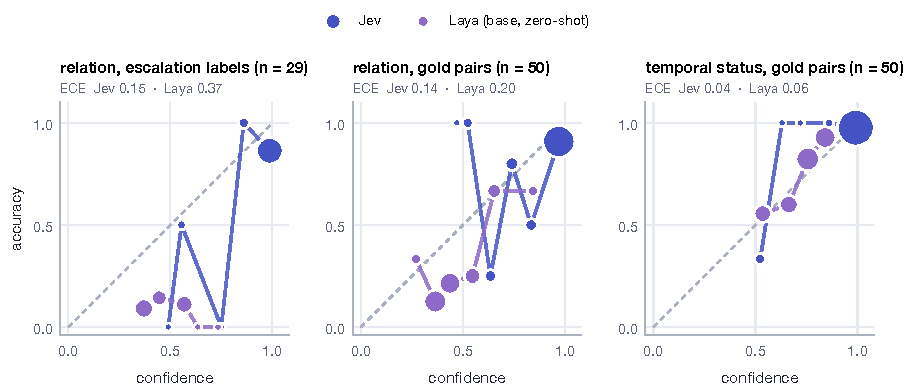
\includegraphics[width=\textwidth]{figures/calibration.pdf}
\caption{reliability diagrams (accuracy against confidence) for Jev and Laya on both label sets.}\label{fig:6}
\end{figure*}
\begin{figure}[!htbp]
\centering
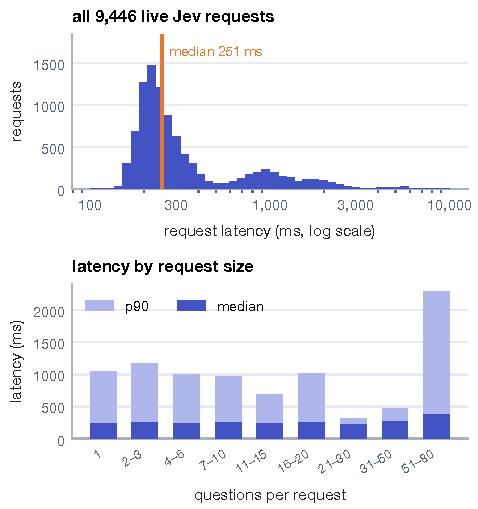
\includegraphics[width=0.6\linewidth]{figures/latency.pdf}
\caption{Jev request latency: distribution over all logged requests, and median and p90 by request size.}\label{fig:7}
\end{figure}
\FloatBarrier
\section{Laya, an open-weights checkpoint (exploratory)}\label{app:D}
\textbf{Laya.} Laya is an open-weights model with the same request format. We ran checkpoint convaiinnovations/laya\src{bench/results/e4\_belief\_v2\_laya\_\_dev\_updates\_\_k3.json} locally through the laya-mlx port on an Apple M2 Pro\src{bench/results/e4\_belief\_v2\_laya\_\_dev\_updates\_\_k3.json} with 32\src{bench/results/e4\_belief\_v2\_laya\_\_dev\_updates\_\_k3.json} GB. It reads at most 512\src{bench/results/e4\_belief\_v2\_laya\_\_dev\_updates\_\_k3.json} tokens per question, of which at most 192\src{bench/results/e4\_belief\_v2\_laya\_\_dev\_updates\_\_k3.json} go to the instructions and options. This is the 421M\src{convai2026laya (model card)} base checkpoint. Its model card reports zero-shot typed-decision accuracy of 0.362\src{convai2026laya (base checkpoint, typed-decisions, zero-shot)} against a 0.318\src{convai2026laya (random baseline)} random baseline, calls it ``a fast base to specialise, not a zero-shot decision engine,'' and offers a separate checkpoint fine-tuned for typed decisions \citep{convai2026laya}. We used the base checkpoint zero-shot.

Everything in this part concerns the 421M\src{convai2026laya (model card)} base checkpoint, used zero-shot as its documentation advises against \citep{convai2026laya}. The checkpoint fine-tuned for typed decisions (reported at 0.766\src{convai2026laya (laya-typed-decisions, fine-tuned)} on its own benchmark) and fine-tuning on our escalation labels were not tested; they are the obvious follow-up.

On the 50\src{bench/results/tradeoff.json} regression pairs (Table~\ref{tab:14}), Laya chooses an accepted relation for 48.0\%\src{bench/results/laya\_regression\_jev\_wording.json} with Jev's question wording and 38.0\%\src{bench/results/laya\_regression\_native.json} with wording rewritten to fit its 192\src{bench/results/e4\_belief\_v2\_laya\_\_dev\_updates\_\_k3.json}-token question budget. Jev scores 90.0\%\src{bench/results/jev\_regression\_v2.json}. Laya never reaches the action threshold, so it closes nothing. Its gold-pair relation accuracy is 28.0\%\src{bench/results/calibration.json} (Table~\ref{tab:15}). A temperature lowers its ECE but not its accuracy.

With the frozen Jev arm replayed from cache and Laya answering every request on the side, the two gave the same answer on 44.8\%\src{bench/results/laya\_agreement.json} of 6,764\src{bench/results/laya\_agreement.json} decisions and the same action at the 0.85\src{src/engram/config.py} threshold on 31.2\%\src{bench/results/laya\_agreement.json}. On \texttt{relation\_\allowbreak{}to\_\allowbreak{}candidate} they agreed on 5.9\%\src{bench/results/laya\_agreement.json} (Table~\ref{tab:16} and Figure~\ref{fig:8}).

When Laya decided every question, on dev + set 1 at $k{=}$3 it scored 24/35\src{bench/results/e4\_belief\_v2\_laya\_\_dev\_updates\_\_k3.json} LoCoMo and 26/30\src{bench/results/e4\_belief\_v2\_laya\_\_dev\_updates\_\_k3.json} update questions. Jev scored 29/35\src{bench/results/e4\_belief\_v2\_shadow\_\_dev\_updates\_\_k3.json} and 30/30\src{bench/results/e4\_belief\_v2\_shadow\_\_dev\_updates\_\_k3.json}. It made 23\src{bench/results/e4\_belief\_v2\_laya\_\_dev\_updates\_\_k3.json} closes, of which 23\src{bench/results/e4\_belief\_v2\_laya\_\_dev\_updates\_\_k3.json} match no labeled pair, and left 43\src{bench/results/e4\_belief\_v2\_laya\_\_dev\_updates\_\_k3.json} of 66\src{bench/results/e4\_belief\_v2\_laya\_\_dev\_updates\_\_k3.json} facts active. Most of these closes came from weak \texttt{duplicate} and \texttt{refinement} answers below 0.5 lowering belief, the failure belief v3 removes \cref{eq:belief}.

\textbf{Hybrid.} In a hybrid arm Laya answered the two high-volume yes/no questions (\texttt{relevant\_\allowbreak{}to\_\allowbreak{}query}, \texttt{same\_\allowbreak{}fact}) and Jev the rest. On the routed questions the two models gave the same answer on 86.9\%\src{bench/results/hybrid\_report.json} and the same action on 34.1\%\src{bench/results/hybrid\_report.json}. Writes were identical to the all-Jev arm, but at $k{=}$3 only 51.8\%\src{bench/results/hybrid\_report.json} of Jev's top-3 lines survived the change of reranker. The hybrid saved 42.6\%\src{bench/results/hybrid\_report.json} of Jev's cost on dev + set 1 (\$0.025\src{bench/results/hybrid\_report.json} per run); Table~\ref{tab:17} has its accuracy.

\begin{table}[!htbp]
\centering
\footnotesize\hyphenpenalty=10000\exhyphenpenalty=10000\setlength{\tabcolsep}{6.0pt}
\caption{Contradiction regression (50\src{bench/results/tradeoff.json} gold pairs), relation\_to\_candidate and temporal\_status in one request. Laya: convaiinnovations/laya\src{bench/results/e4\_belief\_v2\_laya\_\_dev\_updates\_\_k3.json} base checkpoint, zero-shot, fp16, on the local MLX server. Jev chooses an accepted relation for 90.0\%\src{bench/results/jev\_regression\_v2.json} of the pairs with no false close; the Laya base checkpoint chooses one for at most 48.0\%\src{bench/results/laya\_regression\_jev\_wording.json} and never closes.}\label{tab:14}
\begin{tabular}{@{}>{\raggedright\arraybackslash}p{192.0pt}>{\raggedleft\arraybackslash}p{43.3pt}>{\raggedleft\arraybackslash}p{47.8pt}>{\raggedleft\arraybackslash}p{36.0pt}>{\raggedleft\arraybackslash}p{37.9pt}>{\raggedleft\arraybackslash}p{37.9pt}@{}}
\toprule
\textbf{backend} & \textbf{relation exact} & \textbf{temporal} & \textbf{close rule} & \textbf{closes} & \textbf{false closes} \\
\midrule
Jev (jev-1.13.0) & 90.0\%\src{bench/results/jev\_regression\_v2.json} & 94.0\%\src{bench/results/jev\_regression\_v2.json} & 76.0\%\src{bench/results/jev\_regression\_v2.json} & 22\src{bench/results/jev\_regression\_v2.json} & 0\src{bench/results/jev\_regression\_v2.json} \\
Laya, Jev wording (truncated) & 48.0\%\src{bench/results/laya\_regression\_jev\_wording.json} & 76.0\%\src{bench/results/laya\_regression\_jev\_wording.json} & 32.0\%\src{bench/results/laya\_regression\_jev\_wording.json} & 0\src{bench/results/laya\_regression\_jev\_wording.json} & 0\src{bench/results/laya\_regression\_jev\_wording.json} \\
Laya, native wording (fits) & 38.0\%\src{bench/results/laya\_regression\_native.json} & 76.0\%\src{bench/results/laya\_regression\_native.json} & 32.0\%\src{bench/results/laya\_regression\_native.json} & 0\src{bench/results/laya\_regression\_native.json} & 0\src{bench/results/laya\_regression\_native.json} \\
\bottomrule
\end{tabular}
\end{table}
\begingroup\scriptsize
\begin{longtable}{>{\raggedright\arraybackslash}p{0.063\linewidth}>{\raggedright\arraybackslash}p{0.063\linewidth}>{\raggedright\arraybackslash}p{0.063\linewidth}>{\raggedleft\arraybackslash}p{0.063\linewidth}>{\raggedleft\arraybackslash}p{0.063\linewidth}>{\raggedleft\arraybackslash}p{0.063\linewidth}>{\raggedleft\arraybackslash}p{0.063\linewidth}>{\raggedleft\arraybackslash}p{0.063\linewidth}>{\raggedleft\arraybackslash}p{0.063\linewidth}>{\raggedleft\arraybackslash}p{0.067\linewidth}>{\raggedleft\arraybackslash}p{0.067\linewidth}}
\caption{Calibration of the Laya base checkpoint (zero-shot) on the same label sets and with the same measures as Table~\ref{tab:5}.}\label{tab:15}\\
\toprule
\textbf{labels} & \textbf{question} & \textbf{backend} & \textbf{n} & \textbf{top-1 acc.} & \textbf{mean conf.} & \textbf{ECE} & \textbf{fitted $\tau$} & \textbf{ECE at $\tau$} & \textbf{Brier [95\% CI]} & \textbf{NLL [95\% CI]} \\
\midrule
\endfirsthead
\toprule
\textbf{labels} & \textbf{question} & \textbf{backend} & \textbf{n} & \textbf{top-1 acc.} & \textbf{mean conf.} & \textbf{ECE} & \textbf{fitted $\tau$} & \textbf{ECE at $\tau$} & \textbf{Brier [95\% CI]} & \textbf{NLL [95\% CI]} \\
\midrule
\endhead
escalation & relation & laya & 29\src{bench/results/calibration.json} & 10.3\%\src{bench/results/calibration.json} & 0.47\src{bench/results/calibration.json} & 0.37\src{bench/results/calibration.json} & 5.41\src{bench/results/calibration.json} & 0.12\src{bench/results/calibration.json} & 1.00\src{bench/results/calibration\_\allowbreak{}scores.json} [0.90\src{bench/results/calibration\_\allowbreak{}scores.json}, 1.09\src{bench/results/calibration\_\allowbreak{}scores.json}] & 2.11\src{bench/results/calibration\_\allowbreak{}scores.json} [1.83\src{bench/results/calibration\_\allowbreak{}scores.json}, 2.41\src{bench/results/calibration\_\allowbreak{}scores.json}] \\
gold pairs & relation & laya & 50\src{bench/results/calibration.json} & 28.0\%\src{bench/results/calibration.json} & 0.47\src{bench/results/calibration.json} & 0.20\src{bench/results/calibration.json} & 4.22\src{bench/results/calibration.json} & 0.02\src{bench/results/calibration.json} & 0.83\src{bench/results/calibration\_\allowbreak{}scores.json} [0.72\src{bench/results/calibration\_\allowbreak{}scores.json}, 0.94\src{bench/results/calibration\_\allowbreak{}scores.json}] & 1.81\src{bench/results/calibration\_\allowbreak{}scores.json} [1.53\src{bench/results/calibration\_\allowbreak{}scores.json}, 2.09\src{bench/results/calibration\_\allowbreak{}scores.json}] \\
gold pairs & temporal status & laya & 50\src{bench/results/calibration.json} & 76.0\%\src{bench/results/calibration.json} & 0.72\src{bench/results/calibration.json} & 0.06\src{bench/results/calibration.json} & 0.74\src{bench/results/calibration.json} & 0.07\src{bench/results/calibration.json} & 0.33\src{bench/results/calibration\_\allowbreak{}scores.json} [0.22\src{bench/results/calibration\_\allowbreak{}scores.json}, 0.45\src{bench/results/calibration\_\allowbreak{}scores.json}] & 0.57\src{bench/results/calibration\_\allowbreak{}scores.json} [0.44\src{bench/results/calibration\_\allowbreak{}scores.json}, 0.72\src{bench/results/calibration\_\allowbreak{}scores.json}] \\
\bottomrule
\end{longtable}
\endgroup
\begin{table}[!htbp]
\centering
\footnotesize\hyphenpenalty=10000\exhyphenpenalty=10000\setlength{\tabcolsep}{6.0pt}
\caption{Laya against Jev on identical requests: dev + update sets 1 and 2, frozen arm's trajectory at $k{=}$3 (write and retrieval decisions; n per row). Jev jev-1.13.0; Laya base checkpoint, zero-shot. Same action: both choose the same label at $\pi \ge$ 0.85\src{src/engram/config.py}, or neither reaches it. Acts: share of decisions at $\pi \ge$ 0.85\src{src/engram/config.py}.}\label{tab:16}
\begin{tabular}{@{}>{\raggedright\arraybackslash}p{215.4pt}>{\raggedleft\arraybackslash}p{32.2pt}>{\raggedleft\arraybackslash}p{41.7pt}>{\raggedleft\arraybackslash}p{35.4pt}>{\raggedleft\arraybackslash}p{35.2pt}>{\raggedleft\arraybackslash}p{35.2pt}@{}}
\toprule
\textbf{question} & \textbf{n} & \textbf{same answer} & \textbf{same action} & \textbf{Jev acts} & \textbf{Laya acts} \\
\midrule
\texttt{relation\_\allowbreak{}to\_\allowbreak{}candidate} & 2,779\src{bench/results/laya\_agreement.json} & 5.9\%\src{bench/results/laya\_agreement.json} & 18.5\%\src{bench/results/laya\_agreement.json} & 79.9\%\src{bench/results/laya\_agreement.json} & 6.4\%\src{bench/results/laya\_agreement.json} \\
\texttt{relevant\_\allowbreak{}to\_\allowbreak{}query} & 1,440\src{bench/results/laya\_agreement.json} & 93.5\%\src{bench/results/laya\_agreement.json} & 38.9\%\src{bench/results/laya\_agreement.json} & 89.7\%\src{bench/results/laya\_agreement.json} & 31.3\%\src{bench/results/laya\_agreement.json} \\
\texttt{same\_\allowbreak{}fact} & 585\src{bench/results/laya\_agreement.json} & 72.6\%\src{bench/results/laya\_agreement.json} & 35.2\%\src{bench/results/laya\_agreement.json} & 96.2\%\src{bench/results/laya\_agreement.json} & 34.4\%\src{bench/results/laya\_agreement.json} \\
\texttt{plan\_\allowbreak{}fulfilled} & 522\src{bench/results/laya\_agreement.json} & 66.5\%\src{bench/results/laya\_agreement.json} & 16.1\%\src{bench/results/laya\_agreement.json} & 90.0\%\src{bench/results/laya\_agreement.json} & 32.6\%\src{bench/results/laya\_agreement.json} \\
\texttt{worth\_\allowbreak{}remembering} & 226\src{bench/results/laya\_agreement.json} & 53.5\%\src{bench/results/laya\_agreement.json} & 77.0\%\src{bench/results/laya\_agreement.json} & 18.1\%\src{bench/results/laya\_agreement.json} & 4.9\%\src{bench/results/laya\_agreement.json} \\
\texttt{fact\_\allowbreak{}kind} & 226\src{bench/results/laya\_agreement.json} & 41.6\%\src{bench/results/laya\_agreement.json} & 38.1\%\src{bench/results/laya\_agreement.json} & 63.7\%\src{bench/results/laya\_agreement.json} & 15.5\%\src{bench/results/laya\_agreement.json} \\
\texttt{temporal\_\allowbreak{}status} & 226\src{bench/results/laya\_agreement.json} & 66.8\%\src{bench/results/laya\_agreement.json} & 42.5\%\src{bench/results/laya\_agreement.json} & 62.8\%\src{bench/results/laya\_agreement.json} & 5.3\%\src{bench/results/laya\_agreement.json} \\
\texttt{edge\_\allowbreak{}type} & 226\src{bench/results/laya\_agreement.json} & 41.6\%\src{bench/results/laya\_agreement.json} & 50.9\%\src{bench/results/laya\_agreement.json} & 29.2\%\src{bench/results/laya\_agreement.json} & 55.3\%\src{bench/results/laya\_agreement.json} \\
\texttt{durability} & 226\src{bench/results/laya\_agreement.json} & 43.8\%\src{bench/results/laya\_agreement.json} & 47.3\%\src{bench/results/laya\_agreement.json} & 52.7\%\src{bench/results/laya\_agreement.json} & 0.0\%\src{bench/results/laya\_agreement.json} \\
\texttt{sensitivity} & 226\src{bench/results/laya\_agreement.json} & 66.4\%\src{bench/results/laya\_agreement.json} & 57.5\%\src{bench/results/laya\_agreement.json} & 45.1\%\src{bench/results/laya\_agreement.json} & 7.1\%\src{bench/results/laya\_agreement.json} \\
\texttt{query\_\allowbreak{}relation} & 48\src{bench/results/laya\_agreement.json} & 54.2\%\src{bench/results/laya\_agreement.json} & 47.9\%\src{bench/results/laya\_agreement.json} & 39.6\%\src{bench/results/laya\_agreement.json} & 75.0\%\src{bench/results/laya\_agreement.json} \\
\texttt{relation\_\allowbreak{}to\_\allowbreak{}candidate\_\allowbreak{}recheck} & 34\src{bench/results/laya\_agreement.json} & 29.4\%\src{bench/results/laya\_agreement.json} & 41.2\%\src{bench/results/laya\_agreement.json} & 35.3\%\src{bench/results/laya\_agreement.json} & 26.5\%\src{bench/results/laya\_agreement.json} \\
\bottomrule
\end{tabular}
\end{table}
\begin{table}[!htbp]
\centering
\footnotesize\hyphenpenalty=10000\exhyphenpenalty=10000\setlength{\tabcolsep}{6.0pt}
\caption{Hybrid against all-Jev: dev slice with update sets (Q per row: 35\src{bench/results/e2\_jev\_\_dev.json} LoCoMo, 30\src{bench/updates\_conv26.json} set 1, 20\src{bench/updates2\_conv26.json} set 2), k as labeled, extraction claude-haiku-4-5, answers and judge claude-sonnet-4-6.}\label{tab:17}
\begin{tabular}{@{}>{\raggedright\arraybackslash}p{195.6pt}>{\raggedleft\arraybackslash}p{54.5pt}>{\raggedleft\arraybackslash}p{51.3pt}>{\raggedleft\arraybackslash}p{54.5pt}>{\raggedleft\arraybackslash}p{51.3pt}@{}}
\toprule
\textbf{questions} & \textbf{all-Jev $k{=}$3} & \textbf{hybrid $k{=}$3} & \textbf{all-Jev $k{=}$20} & \textbf{hybrid $k{=}$20} \\
\midrule
update set 1 & 30/30\src{bench/results/e4\_belief\_v2\_shadow\_\_dev\_updates\_\_k3.json} & 27/30\src{bench/results/e4\_belief\_v2\_hybrid\_\_dev\_updates\_\_k3.json} & 30/30\src{bench/results/e4\_belief\_v2\_shadow\_\_dev\_updates\_\_k20.json} & 30/30\src{bench/results/e4\_belief\_v2\_hybrid\_\_dev\_updates\_\_k20.json} \\
LoCoMo dev & 29/35\src{bench/results/e4\_belief\_v2\_shadow\_\_dev\_updates\_\_k3.json} & 29/35\src{bench/results/e4\_belief\_v2\_hybrid\_\_dev\_updates\_\_k3.json} & 31/35\src{bench/results/e4\_belief\_v2\_shadow\_\_dev\_updates\_\_k20.json} & 31/35\src{bench/results/e4\_belief\_v2\_hybrid\_\_dev\_updates\_\_k20.json} \\
update set 2 & 19/20\src{bench/results/e4\_belief\_v2\_shadow\_\_dev\_updates2\_\_k3.json} & 17/20\src{bench/results/e4\_belief\_v2\_hybrid\_\_dev\_updates2\_\_k3.json} & 20/20\src{bench/results/e4\_belief\_v2\_shadow\_\_dev\_updates2\_\_k20.json} & 20/20\src{bench/results/e4\_belief\_v2\_hybrid\_\_dev\_updates2\_\_k20.json} \\
\bottomrule
\end{tabular}
\end{table}
\begin{figure}[!htbp]
\centering
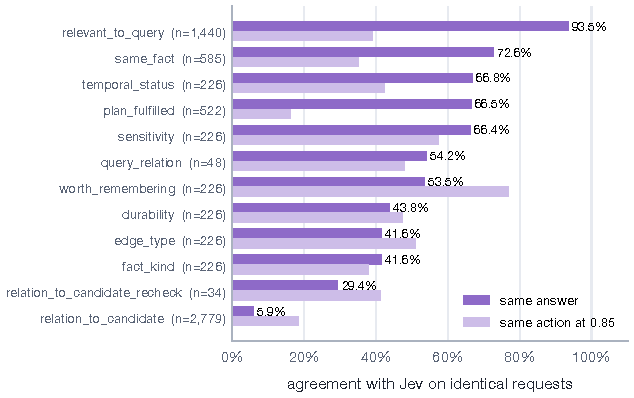
\includegraphics[width=0.6\linewidth]{figures/laya_agreement.pdf}
\caption{Agreement between the Laya base checkpoint (zero-shot) and Jev on identical requests, per question, sorted by same answer. Dev + update sets 1 and 2, frozen arm's trajectory.}\label{fig:8}
\end{figure}
\FloatBarrier
\section{Reproduction}\label{app:E}
Each table and figure was produced by the command below, run from the root of the engram codebase. With the call cache (\texttt{bench/\allowbreak{}.cache/\allowbreak{}calls.sqlite}) in place, every command in Table~\ref{tab:18} replays at no API cost.

\begingroup\scriptsize
\begin{longtable}{>{\raggedright\arraybackslash}p{0.298\linewidth}>{\raggedright\arraybackslash}p{0.639\linewidth}}
\caption{The command behind each table and figure.}\label{tab:18}\\
\toprule
\textbf{table / figure} & \textbf{command} \\
\midrule
\endfirsthead
\toprule
\textbf{table / figure} & \textbf{command} \\
\midrule
\endhead
Table~\ref{tab:1} & \texttt{python -m bench.run -{}-arm \{e2\_\allowbreak{}\allowbreak{}jev,e2\_\allowbreak{}\allowbreak{}llm,mem0\} -{}-slice dev} \\
Tables~\ref{tab:2}, \ref{tab:3}, \ref{tab:8}--\ref{tab:10}; Fig.~\ref{fig:2} & \texttt{python -m bench.run -{}-arm \{e4\_\allowbreak{}\allowbreak{}belief\_\allowbreak{}\allowbreak{}v2,mem0\} -{}-slice heldout:\textless{}conv\textgreater{} -{}-top-k 3 -{}-also-top-k 20}, then \texttt{python -m bench.heldout\_\allowbreak{}\allowbreak{}report}, \texttt{python -m bench.token\_\allowbreak{}\allowbreak{}match}, \texttt{python -m bench.perconv} and \texttt{python -m bench.heldout\_\allowbreak{}\allowbreak{}extra} (reranking off, adversarial) \\
\Cref{sec:4.2} & \texttt{python -m bench.e2\_\allowbreak{}\allowbreak{}extraction\_\allowbreak{}\allowbreak{}diff} \\
Table~\ref{tab:4}; Figs.~\ref{fig:3}, \ref{fig:4} & \texttt{python -m bench.run -{}-arm \textless{}arm\textgreater{} -{}-slice dev\_\allowbreak{}\allowbreak{}updates[2] [-{}-top-k 3] [-{}-no-dates]} \\
Tables~\ref{tab:5}, \ref{tab:14}, \ref{tab:15}; Figs.~\ref{fig:6}, \ref{fig:8} & \texttt{python bench/\allowbreak{}test\_\allowbreak{}\allowbreak{}contradictions.py -{}-backend laya [-{}-native] -{}-save \ldots{}}, \texttt{python -m bench.calibration}, \texttt{python -m bench.calibration\_\allowbreak{}\allowbreak{}scores}, \texttt{python -m bench.jev\_\allowbreak{}\allowbreak{}regression} (the Laya rows need \texttt{bench/\allowbreak{}laya\_\allowbreak{}\allowbreak{}server.py} running) \\
Fig.~\ref{fig:5} & \texttt{python -m bench.tradeoff} \\
Tables~\ref{tab:16}, \ref{tab:17} & \texttt{python -m bench.laya\_\allowbreak{}\allowbreak{}report}, \texttt{python -m bench.hybrid\_\allowbreak{}\allowbreak{}report} \\
Table~\ref{tab:11}, Fig.~\ref{fig:7} & \texttt{python -m bench.jev\_\allowbreak{}\allowbreak{}latency} \\
Table~\ref{tab:13}; \cref{sec:5.5} read path & \texttt{python -m bench.read\_\allowbreak{}\allowbreak{}path} \\
this paper & \texttt{python paper/\allowbreak{}build.py}, \texttt{python paper/\allowbreak{}figures.py} \\
\bottomrule
\end{longtable}
\endgroup
The spend ledger records cost per run, not per table; Table~\ref{tab:19} gives per-arm totals.

\begingroup\scriptsize
\begin{longtable}{>{\raggedright\arraybackslash}p{0.269\linewidth}>{\raggedleft\arraybackslash}p{0.205\linewidth}>{\raggedleft\arraybackslash}p{0.205\linewidth}>{\raggedleft\arraybackslash}p{0.205\linewidth}}
\caption{Phase 2 spend per arm, in USD (\texttt{bench/\allowbreak{}results/\allowbreak{}phase2\_\allowbreak{}spend.jsonl}).}\label{tab:19}\\
\toprule
\textbf{arm} & \textbf{runs} & \textbf{Jev} & \textbf{Claude} \\
\midrule
\endfirsthead
\toprule
\textbf{arm} & \textbf{runs} & \textbf{Jev} & \textbf{Claude} \\
\midrule
\endhead
\texttt{mem0} & 15\src{bench/results/phase2\_\allowbreak{}spend.jsonl} & \$0.0000\src{bench/results/phase2\_\allowbreak{}spend.jsonl} & \$35.94\src{bench/results/phase2\_\allowbreak{}spend.jsonl} \\
\texttt{e4\_\allowbreak{}\allowbreak{}belief\_\allowbreak{}\allowbreak{}v2} & 18\src{bench/results/phase2\_\allowbreak{}spend.jsonl} & \$1.0917\src{bench/results/phase2\_\allowbreak{}spend.jsonl} & \$31.80\src{bench/results/phase2\_\allowbreak{}spend.jsonl} \\
\texttt{heldout\_\allowbreak{}\allowbreak{}extra} & 4\src{bench/results/phase2\_\allowbreak{}spend.jsonl} & \$0.0365\src{bench/results/phase2\_\allowbreak{}spend.jsonl} & \$8.50\src{bench/results/phase2\_\allowbreak{}spend.jsonl} \\
\texttt{e2\_\allowbreak{}\allowbreak{}jev} & 2\src{bench/results/phase2\_\allowbreak{}spend.jsonl} & \$0.0636\src{bench/results/phase2\_\allowbreak{}spend.jsonl} & \$3.51\src{bench/results/phase2\_\allowbreak{}spend.jsonl} \\
\texttt{e2\_\allowbreak{}\allowbreak{}llm} & 2\src{bench/results/phase2\_\allowbreak{}spend.jsonl} & \$0.0134\src{bench/results/phase2\_\allowbreak{}spend.jsonl} & \$3.21\src{bench/results/phase2\_\allowbreak{}spend.jsonl} \\
\texttt{mem0\_\allowbreak{}\allowbreak{}token\_\allowbreak{}\allowbreak{}matched} & 1\src{bench/results/phase2\_\allowbreak{}spend.jsonl} & \$0.0000\src{bench/results/phase2\_\allowbreak{}spend.jsonl} & \$2.52\src{bench/results/phase2\_\allowbreak{}spend.jsonl} \\
\texttt{e4\_\allowbreak{}\allowbreak{}belief\_\allowbreak{}\allowbreak{}v2\_\allowbreak{}\allowbreak{}laya} & 2\src{bench/results/phase2\_\allowbreak{}spend.jsonl} & \$0.0405\src{bench/results/phase2\_\allowbreak{}spend.jsonl} & \$2.40\src{bench/results/phase2\_\allowbreak{}spend.jsonl} \\
\texttt{e2\_\allowbreak{}\allowbreak{}jev\_\allowbreak{}\allowbreak{}v2} & 4\src{bench/results/phase2\_\allowbreak{}spend.jsonl} & \$0.0362\src{bench/results/phase2\_\allowbreak{}spend.jsonl} & \$2.35\src{bench/results/phase2\_\allowbreak{}spend.jsonl} \\
\texttt{e1\_\allowbreak{}\allowbreak{}recall} & 4\src{bench/results/phase2\_\allowbreak{}spend.jsonl} & \$0.0653\src{bench/results/phase2\_\allowbreak{}spend.jsonl} & \$2.05\src{bench/results/phase2\_\allowbreak{}spend.jsonl} \\
\texttt{e4\_\allowbreak{}\allowbreak{}belief} & 6\src{bench/results/phase2\_\allowbreak{}spend.jsonl} & \$0.0316\src{bench/results/phase2\_\allowbreak{}spend.jsonl} & \$1.69\src{bench/results/phase2\_\allowbreak{}spend.jsonl} \\
\texttt{e3\_\allowbreak{}\allowbreak{}structural\_\allowbreak{}\allowbreak{}v2} & 1\src{bench/results/phase2\_\allowbreak{}spend.jsonl} & \$0.0278\src{bench/results/phase2\_\allowbreak{}spend.jsonl} & \$1.44\src{bench/results/phase2\_\allowbreak{}spend.jsonl} \\
\texttt{e0\_\allowbreak{}\allowbreak{}baseline} & 8\src{bench/results/phase2\_\allowbreak{}spend.jsonl} & \$0.0736\src{bench/results/phase2\_\allowbreak{}spend.jsonl} & \$1.36\src{bench/results/phase2\_\allowbreak{}spend.jsonl} \\
\texttt{mem0\_\allowbreak{}\allowbreak{}dated} & 1\src{bench/results/phase2\_\allowbreak{}spend.jsonl} & \$0.0000\src{bench/results/phase2\_\allowbreak{}spend.jsonl} & \$0.96\src{bench/results/phase2\_\allowbreak{}spend.jsonl} \\
\texttt{e3\_\allowbreak{}\allowbreak{}structural\_\allowbreak{}\allowbreak{}v3} & 2\src{bench/results/phase2\_\allowbreak{}spend.jsonl} & \$0.0272\src{bench/results/phase2\_\allowbreak{}spend.jsonl} & \$0.76\src{bench/results/phase2\_\allowbreak{}spend.jsonl} \\
\texttt{e4\_\allowbreak{}\allowbreak{}belief\_\allowbreak{}\allowbreak{}v2\_\allowbreak{}\allowbreak{}hybrid} & 4\src{bench/results/phase2\_\allowbreak{}spend.jsonl} & \$0.0000\src{bench/results/phase2\_\allowbreak{}spend.jsonl} & \$0.73\src{bench/results/phase2\_\allowbreak{}spend.jsonl} \\
\texttt{e4\_\allowbreak{}\allowbreak{}belief\_\allowbreak{}\allowbreak{}v2\_\allowbreak{}\allowbreak{}compact} & 2\src{bench/results/phase2\_\allowbreak{}spend.jsonl} & \$0.0000\src{bench/results/phase2\_\allowbreak{}spend.jsonl} & \$0.59\src{bench/results/phase2\_\allowbreak{}spend.jsonl} \\
\texttt{e4\_\allowbreak{}\allowbreak{}belief\_\allowbreak{}\allowbreak{}v2\_\allowbreak{}\allowbreak{}norerank} & 1\src{bench/results/phase2\_\allowbreak{}spend.jsonl} & \$0.0000\src{bench/results/phase2\_\allowbreak{}spend.jsonl} & \$0.25\src{bench/results/phase2\_\allowbreak{}spend.jsonl} \\
\texttt{e4\_\allowbreak{}\allowbreak{}belief\_\allowbreak{}\allowbreak{}v2\_\allowbreak{}\allowbreak{}shadow} & 2\src{bench/results/phase2\_\allowbreak{}spend.jsonl} & \$0.0000\src{bench/results/phase2\_\allowbreak{}spend.jsonl} & \$0.18\src{bench/results/phase2\_\allowbreak{}spend.jsonl} \\
\texttt{e3\_\allowbreak{}\allowbreak{}structural} & 1\src{bench/results/phase2\_\allowbreak{}spend.jsonl} & \$0.0008\src{bench/results/phase2\_\allowbreak{}spend.jsonl} & \$0.04\src{bench/results/phase2\_\allowbreak{}spend.jsonl} \\
\texttt{e4\_\allowbreak{}\allowbreak{}belief\_\allowbreak{}\allowbreak{}v2\_\allowbreak{}\allowbreak{}nohist} & 1\src{bench/results/phase2\_\allowbreak{}spend.jsonl} & \$0.0000\src{bench/results/phase2\_\allowbreak{}spend.jsonl} & \$0.01\src{bench/results/phase2\_\allowbreak{}spend.jsonl} \\
\texttt{e4\_\allowbreak{}\allowbreak{}belief\_\allowbreak{}\allowbreak{}v3} & 3\src{bench/results/phase2\_\allowbreak{}spend.jsonl} & \$0.0004\src{bench/results/phase2\_\allowbreak{}spend.jsonl} & \$0.00\src{bench/results/phase2\_\allowbreak{}spend.jsonl} \\
\bottomrule
\end{longtable}
\endgroup
\FloatBarrier
\end{document}